\documentclass[
  man,
  floatsintext,
  longtable,
  nolmodern,
  notxfonts,
  notimes,
  colorlinks=true,linkcolor=blue,citecolor=blue,urlcolor=blue]{apa7}

\usepackage{amsmath}
\usepackage{amssymb}




\RequirePackage{longtable}
\RequirePackage{threeparttablex}

\makeatletter
\renewcommand{\paragraph}{\@startsection{paragraph}{4}{\parindent}%
	{0\baselineskip \@plus 0.2ex \@minus 0.2ex}%
	{-.5em}%
	{\normalfont\normalsize\bfseries\typesectitle}}

\renewcommand{\subparagraph}[1]{\@startsection{subparagraph}{5}{0.5em}%
	{0\baselineskip \@plus 0.2ex \@minus 0.2ex}%
	{-\z@\relax}%
	{\normalfont\normalsize\bfseries\itshape\hspace{\parindent}{#1}\textit{\addperi}}{\relax}}
\makeatother




\usepackage{longtable, booktabs, multirow, multicol, colortbl, hhline, caption, array, float, xpatch}
\usepackage{subcaption}


\renewcommand\thesubfigure{\Alph{subfigure}}
\setcounter{topnumber}{2}
\setcounter{bottomnumber}{2}
\setcounter{totalnumber}{4}
\renewcommand{\topfraction}{0.85}
\renewcommand{\bottomfraction}{0.85}
\renewcommand{\textfraction}{0.15}
\renewcommand{\floatpagefraction}{0.7}

\usepackage{tcolorbox}
\tcbuselibrary{listings,theorems, breakable, skins}
\usepackage{fontawesome5}

\definecolor{quarto-callout-color}{HTML}{909090}
\definecolor{quarto-callout-note-color}{HTML}{0758E5}
\definecolor{quarto-callout-important-color}{HTML}{CC1914}
\definecolor{quarto-callout-warning-color}{HTML}{EB9113}
\definecolor{quarto-callout-tip-color}{HTML}{00A047}
\definecolor{quarto-callout-caution-color}{HTML}{FC5300}
\definecolor{quarto-callout-color-frame}{HTML}{ACACAC}
\definecolor{quarto-callout-note-color-frame}{HTML}{4582EC}
\definecolor{quarto-callout-important-color-frame}{HTML}{D9534F}
\definecolor{quarto-callout-warning-color-frame}{HTML}{F0AD4E}
\definecolor{quarto-callout-tip-color-frame}{HTML}{02B875}
\definecolor{quarto-callout-caution-color-frame}{HTML}{FD7E14}

%\newlength\Oldarrayrulewidth
%\newlength\Oldtabcolsep


\usepackage{hyperref}




\providecommand{\tightlist}{%
  \setlength{\itemsep}{0pt}\setlength{\parskip}{0pt}}
\usepackage{longtable,booktabs,array}
\usepackage{calc} % for calculating minipage widths
% Correct order of tables after \paragraph or \subparagraph
\usepackage{etoolbox}
\makeatletter
\patchcmd\longtable{\par}{\if@noskipsec\mbox{}\fi\par}{}{}
\makeatother
% Allow footnotes in longtable head/foot
\IfFileExists{footnotehyper.sty}{\usepackage{footnotehyper}}{\usepackage{footnote}}
\makesavenoteenv{longtable}

\usepackage{graphicx}
\makeatletter
\newsavebox\pandoc@box
\newcommand*\pandocbounded[1]{% scales image to fit in text height/width
  \sbox\pandoc@box{#1}%
  \Gscale@div\@tempa{\textheight}{\dimexpr\ht\pandoc@box+\dp\pandoc@box\relax}%
  \Gscale@div\@tempb{\linewidth}{\wd\pandoc@box}%
  \ifdim\@tempb\p@<\@tempa\p@\let\@tempa\@tempb\fi% select the smaller of both
  \ifdim\@tempa\p@<\p@\scalebox{\@tempa}{\usebox\pandoc@box}%
  \else\usebox{\pandoc@box}%
  \fi%
}
% Set default figure placement to htbp
\def\fps@figure{htbp}
\makeatother


% definitions for citeproc citations
\NewDocumentCommand\citeproctext{}{}
\NewDocumentCommand\citeproc{mm}{%
  \begingroup\def\citeproctext{#2}\cite{#1}\endgroup}
\makeatletter
 % allow citations to break across lines
 \let\@cite@ofmt\@firstofone
 % avoid brackets around text for \cite:
 \def\@biblabel#1{}
 \def\@cite#1#2{{#1\if@tempswa , #2\fi}}
\makeatother
\newlength{\cslhangindent}
\setlength{\cslhangindent}{1.5em}
\newlength{\csllabelwidth}
\setlength{\csllabelwidth}{3em}
\newenvironment{CSLReferences}[2] % #1 hanging-indent, #2 entry-spacing
 {\begin{list}{}{%
  \setlength{\itemindent}{0pt}
  \setlength{\leftmargin}{0pt}
  \setlength{\parsep}{0pt}
  % turn on hanging indent if param 1 is 1
  \ifodd #1
   \setlength{\leftmargin}{\cslhangindent}
   \setlength{\itemindent}{-1\cslhangindent}
  \fi
  % set entry spacing
  \setlength{\itemsep}{#2\baselineskip}}}
 {\end{list}}
\usepackage{calc}
\newcommand{\CSLBlock}[1]{\hfill\break\parbox[t]{\linewidth}{\strut\ignorespaces#1\strut}}
\newcommand{\CSLLeftMargin}[1]{\parbox[t]{\csllabelwidth}{\strut#1\strut}}
\newcommand{\CSLRightInline}[1]{\parbox[t]{\linewidth - \csllabelwidth}{\strut#1\strut}}
\newcommand{\CSLIndent}[1]{\hspace{\cslhangindent}#1}



% \usepackage{newtx}

% \defaultfontfeatures{Scale=MatchLowercase}
% \defaultfontfeatures[\rmfamily]{Ligatures=TeX,Scale=1}





\title{From screens to words:\\ Exploring family media ecology and
language outcomes in infancy}


\shorttitle{Family media ecology and language in infancy}


\usepackage{etoolbox}









\authorsnames[{1*},{2},{1,3},{4},{4},{5},{6+},{3+}]{Nevena Dimitrova,Alvin
W. M. Tan,Jalisse Schmid,Eleonora Benecchi,Petra Mazzoni,Margarete
Bolten,Fabio Sticca,Eva Unternaehrer}







\authorsaffiliations{
{Faculty of Social Work (HETSL), University of Applied Sciences and Arts
Western Switzerland (HES-SO)},{Department of Psychology, Stanford
University},{Child and Adolescent Psychiatric Research Department,
University Psychiatric Clinics Basel (UPK), University of
Basel},{Institute of Media and Journalism (IMeG), Università della
Svizzera Italiana (USI)},{Luzerner Psychiatrie AG, Clinic for Child and
Adolescent Psychiatry and Children's Hospital of Central Switzerland
(KidZ)},{University of Teacher Education in Special Needs (HfH)}}


\leftheader{Dimitrova, Tan, Schmid, Benecchi, Mazzoni, Bolten, Sticca and Unternaehrer}



\abstract{This study applies the Dynamic, Relational, Ecological
Approach to Media Effects Research (DREAMER) framework to investigate
how family media ecology associates with early vocabulary development.
Drawing on a sample of 279 Swiss families with children aged 8--30
months, we examined how individual (child age, gender), structural
(parental education, daycare attendance, siblings), and contextual
(parental motivations, co-viewing behaviors) factors shape screen use
dynamics and language outcomes. Using a Bayesian structural equation
modeling approach, we tested a serial mediation model linking these
variables to vocabulary percentiles derived from the MacArthur-Bates
Communicative Development Inventory. While structural factors such as
daycare attendance and sibling presence did not predict vocabulary
outcomes, parental motivations---particularly for learning and
behavioral management---were associated with screen use patterns and
co-viewing behaviors. However, these contextual factors did not reliably
predict vocabulary scores. Our findings highlight the complexity of
media effects in early childhood and underscore the importance of
considering developmental timing, family context, and parental intent.
The results support the DREAMER framework's emphasis on dynamic,
bidirectional processes and call for longitudinal, multi-informant
research to better capture the nuanced pathways linking digital media
use to developmental outcomes. }

\keywords{early language development, digital media use, parental
motivations, family media ecology, DREAMER framework}

\authornote{\par{ \textsuperscript{*}Corresponding author}
\par { \textsuperscript{+}Shared last authorship }
\par{\addORCIDlink{Nevena
Dimitrova}{0000-0002-3433-096X}}\par{\addORCIDlink{Alvin W. M. Tan}{0000-0001-5551-7507}}\par{\addORCIDlink{Jalisse
Schmid}{0009-0008-4858-3125}}\par{\addORCIDlink{Eleonora
Benecchi}{0000-0002-8147-7147}}\par{\addORCIDlink{Petra
Mazzoni}{0000-0001-5120-8969}}\par{\addORCIDlink{Margarete
Bolten}{0000-0001-9273-5845}}\par{\addORCIDlink{Fabio
Sticca}{0000-0003-3246-5833}}\par{\addORCIDlink{Eva
Unternaehrer}{0000-0002-3507-1883}} 
\par{ }
\par{ \textbf{Data availability.} The dataset is available upon request addressed to the
corresponding author.}    
\par{ \textbf{Acknowledgements.} We thank all the parents who completed the
SWIPE survey and all institutions that supported distribution of the
survey link. This study was financially supported by: Federal Social
Insurance Office (BSV), Foundation Action Innocence, Fondation Sana,
Haute école de travail social et de la santé Lausanne, HES-SO (HETSL),
and Pädagogische Hochschule Thurgau (PHTG). EU was financially supported
by the research Fund Junior Researchers of the University of Basel,
Grant/Award Number: 3MS1064. None of the funding sources had a role in
the study design, analysis of data, interpretation of results, or
writing of the report. The authors declare no conflict of interest in
the conduct and reporting of research. Generative Artificial
Intelligence was employed to assist with the rephrasing and
summarization of written text, with the full approval of all
authors. }
\par { \textbf{CRediT statement.}  ND: conceptualization (lead); project administration (lead); writing -- original draft (lead); methodology (supporting); formal analysis (supporting); funding acquisition (lead). AWMT: writing -- review and editing (supporting); data curation (lead); formal analysis (lead). JS: data collection (lead), methodology (supporting), data processing (supporting), writing -- review and editing (supporting). EB and PM: writing -- original draft (supporting); writing -- review and editing (supporting); methodology (supporting). MB: writing -- review and editing (supporting); methodology (supporting). FS and EU: conceptualization (lead); project administration (lead); methodology (lead); formal analysis (supporting); funding acquisition (supporting).}

}

\makeatletter
\let\endoldlt\endlongtable
\def\endlongtable{
\hline
\endoldlt
}
\makeatother

\urlstyle{same}



\usepackage{booktabs}
\usepackage{caption}
\usepackage{longtable}
\usepackage{colortbl}
\usepackage{array}
\usepackage{anyfontsize}
\usepackage{multirow}
\renewcommand{\textfraction}{0.0}
\renewcommand{\topfraction}{1}
\renewcommand{\bottomfraction}{1}
\renewcommand{\floatpagefraction}{1}
\makeatletter
\@ifpackageloaded{caption}{}{\usepackage{caption}}
\AtBeginDocument{%
\ifdefined\contentsname
  \renewcommand*\contentsname{Table of contents}
\else
  \newcommand\contentsname{Table of contents}
\fi
\ifdefined\listfigurename
  \renewcommand*\listfigurename{List of Figures}
\else
  \newcommand\listfigurename{List of Figures}
\fi
\ifdefined\listtablename
  \renewcommand*\listtablename{List of Tables}
\else
  \newcommand\listtablename{List of Tables}
\fi
\ifdefined\figurename
  \renewcommand*\figurename{Figure}
\else
  \newcommand\figurename{Figure}
\fi
\ifdefined\tablename
  \renewcommand*\tablename{Table}
\else
  \newcommand\tablename{Table}
\fi
}
\@ifpackageloaded{float}{}{\usepackage{float}}
\floatstyle{ruled}
\@ifundefined{c@chapter}{\newfloat{codelisting}{h}{lop}}{\newfloat{codelisting}{h}{lop}[chapter]}
\floatname{codelisting}{Listing}
\newcommand*\listoflistings{\listof{codelisting}{List of Listings}}
\makeatother
\makeatletter
\makeatother
\makeatletter
\@ifpackageloaded{caption}{}{\usepackage{caption}}
\@ifpackageloaded{subcaption}{}{\usepackage{subcaption}}
\makeatother

% From https://tex.stackexchange.com/a/645996/211326
%%% apa7 doesn't want to add appendix section titles in the toc
%%% let's make it do it
\makeatletter
\xpatchcmd{\appendix}
  {\par}
  {\addcontentsline{toc}{section}{\@currentlabelname}\par}
  {}{}
\makeatother

%% Disable longtable counter
%% https://tex.stackexchange.com/a/248395/211326

\usepackage{etoolbox}

\makeatletter
\patchcmd{\LT@caption}
  {\bgroup}
  {\bgroup\global\LTpatch@captiontrue}
  {}{}
\patchcmd{\longtable}
  {\par}
  {\par\global\LTpatch@captionfalse}
  {}{}
\apptocmd{\endlongtable}
  {\ifLTpatch@caption\else\addtocounter{table}{-1}\fi}
  {}{}
\newif\ifLTpatch@caption
\makeatother

\begin{document}

\maketitle



\setcounter{secnumdepth}{-\maxdimen} % remove section numbering

\setlength\LTleft{0pt}



\vspace{1em}
\section{Introduction}\label{introduction}

Many children under the age of three years are frequent users of digital
screen media (\citeproc{ref-mannCommonSenseCensus2025}{Mann et al.,
2025}; \citeproc{ref-schmidDigitalMediaUse2025}{Schmid et al., 2025}),
despite recommendations against any screen use in young children
(\citeproc{ref-worldhealthorganizationGuidelinesPhysicalActivity2019}{World
Health Organization, 2019}). Given the potential undesirable effects of
screen time on child development
(\citeproc{ref-sticcaScreenDevelopmentSystematic2025}{Sticca et al.,
2025}), understanding how early screen use influences development,
particularly language acquisition, is crucial. While recent studies have
examined links between screen time and language development alongside
other predictors or moderators (e.g.,
\citeproc{ref-bergmannYoungChildrensScreen2022}{Bergmann et al., 2022};
\citeproc{ref-xieScreenExposureBeneficial2024}{Xie et al., 2024}), such
approaches remain largely fragmented. To better understand how screen
use influences development, integrative models are needed that consider
the structural, motivational, and contextual pathways involved
(\citeproc{ref-barrMediaExposureInfancy2017}{Barr \& Linebarger, 2017};
\citeproc{ref-christakisHowEarlyMedia2018}{Christakis et al., 2018};
\citeproc{ref-madiganAssociationScreenTime2019}{Madigan et al., 2019}).
This study applies the \emph{Dynamic, Relational, Ecological Approach to
Media Effects Research} framework (DREAMER;
\citeproc{ref-barrEarlyChildhoodDigital2024}{Barr et al., 2024}) to
propose a four-step model linking early digital media use to vocabulary
development within the broader family media context. Specifically, we
investigate how individual and structural factors influence parents'
motivations for allowing child screen use; how, in turn, these
motivations relate to young children's screen use patterns; and,
ultimately, how early screen exposure is associated with vocabulary
development in children under the age of three years.

Understanding how screen-based digital media use impacts infant
development is crucial due to the neurodevelopmental sensitivity in
early childhood
(\citeproc{ref-christakisEffectsInfantMedia2009}{Christakis, 2009}) and
the growing ubiquity of screens in family life. Early screen‐use habits
often persist, underscoring the need for research to inform best
practices and policy even in young children
(\citeproc{ref-aapcounciloncommunicationsandmediaMediaYoungMinds2016}{AAP
Council on Communications and Media et al., 2016};
\citeproc{ref-madiganAssociationScreenTime2019}{Madigan et al., 2019}).
Of various developmental outcomes, language is particularly vital: It
depends on interactive, contingent exchanges that screens typically lack
(\citeproc{ref-roseberrySkypeMeSocially2014}{Roseberry et al., 2014};
\citeproc{ref-zimmermanAssociationsMediaViewing2007}{Zimmerman et al.,
2007}) and serves as both a key developmental milestone and a foundation
for later cognitive, social, and academic success
(\citeproc{ref-hirsh-pasekPuttingEducationEducational2015}{Hirsh-Pasek
et al., 2015}).

The use of digital screens in the early years is widespread
(\citeproc{ref-mannCommonSenseCensus2025}{Mann et al., 2025}) and may
displace opportunities for rich, interactive experiences that are
foundational to early psychological development
(\citeproc{ref-oswaldPsychologicalImpactsScreen2020}{Oswald et al.,
2020}). Studies have reported that children with higher amounts of
screen use tend to have lower language abilities, and decreased
vocabulary in particular, both when screen use and vocabulary size are
measured concurrently (\citeproc{ref-jingScreenMediaExposure2023}{Jing
et al., 2023}; \citeproc{ref-madiganAssociationScreenTime2019}{Madigan
et al., 2019}) and longitudinally
(\citeproc{ref-sundqvistLongitudinalStudyRelationship2024}{Sundqvist et
al., 2024}).

Recent research has moved beyond screen time alone, recognizing that it
does not fully capture the ways in which screen media influence
children's language development. Contemporary research reveals that
digital media effects are not uniform but depend critically on
individual and structural factors, on digital media dynamics such as
parental reasons and motivations for child screen use, as well as on the
characteristics of the child's screen use in terms of the content and
the context of screen exposure.

\subsection{Individual and structural factors shaping screen--language
relationships}\label{individual-and-structural-factors-shaping-screenlanguage-relationships}

The relationship between screen use and language development operates
within a complex web of individual and structural factors that both
predict screen exposure patterns and moderate their developmental
impact. Child age serves as a primary predictor of screen exposure, with
screen time increasing as children grow older
(\citeproc{ref-mannCommonSenseCensus2025}{Mann et al., 2025};
\citeproc{ref-schmidDigitalMediaUse2025}{Schmid et al., 2025}).
Importantly, age also functions as a critical moderator of
screen-related risks. Early exposure during toddlerhood (12--30 months)
is associated with elevated risks of language delays, while moderate
exposure among older toddlers (31--48 months) demonstrates fewer
negative associations
(\citeproc{ref-chakhunashviliDoesScreenTime2024}{Chakhunashvili et al.,
2024}). Regarding gender, although girls typically demonstrate slightly
stronger early vocabulary development, excessive screen use negatively
impacts language development across genders, particularly when
interactive, co-viewed content is absent
(\citeproc{ref-tulvisteWeekendScreenUse2024}{Tulviste \& Tulviste,
2024}).

Structural factors create both direct and indirect pathways to
screen-language relationships. Lower-income families report higher
levels of screen exposure
(\citeproc{ref-anandDemographicPredictorsMedia2005}{Anand \& Krosnick,
2005}; \citeproc{ref-calvertAgeEthnicitySocioeconomic2005}{Calvert et
al., 2005}), while income also moderates developmental outcomes
(\citeproc{ref-linverFamilyProcessesPathways2002}{Linver et al., 2002};
\citeproc{ref-schwabLanguageLearningSocioeconomic2016}{Schwab \&
Lew-Williams, 2016}). Children from lower socioeconomic backgrounds are
more likely to experience screen use without enriching caregiver
interaction, which can substantially undermine language development
(\citeproc{ref-balExaminingRelationshipLanguage2024}{Bal et al., 2024}).
Similarly, parental education level significantly influences both screen
exposure patterns and mediation strategies. For instance, parents with
lower educational attainment tend to permit more passive screen use
(\citeproc{ref-mannCommonSenseCensus2025}{Mann et al., 2025}), 
whereas higher-educated parents are more likely to engage in
co-viewing and support language development through interactive media
practices (\citeproc{ref-ponsMaternalEducationLevel2020}{Pons et al.,
2020}).

\subsection{Parental motivations: The hidden driver of language
outcomes}\label{parental-motivations-the-hidden-driver-of-language-outcomes}

Parental motivations underlying child screen use significantly influence
language development outcomes, often in ways that contradict intended
benefits. Parents commonly report using digital media to keep their
child entertained while they are occupied, to take a break from
caregiving, or to help regulate their child's behavior or emotional
state (\citeproc{ref-nikkenParentsInstrumentalUse2019}{Nikken, 2019}).
When screens serve convenience purposes---such as behavioral management
or parental respite---language outcomes potentially suffer due to
reduced caregiver--child interaction
(\citeproc{ref-madiganAssociationScreenTime2019}{Madigan et al., 2019}).
While some parents emphasize learning and creativity as primary
motivations for child screen use
(\citeproc{ref-schmidDigitalMediaUse2025}{Schmid et al., 2025}),
educational intentions alone do not guarantee improved outcomes without
accompanying active co-viewing strategies. Convenience-driven screen use
tends to reinforce passive consumption patterns, thus potentially
displacing the conversational exchanges essential for language
acquisition (\citeproc{ref-alroqiAssociationScreenMedia2023}{Alroqi et
al., 2023}; \citeproc{ref-doreCharacteristicsChildrensMedia2020}{Dore et
al., 2020};
\citeproc{ref-strouseEffectiveCoviewingPreschoolers2013}{Strouse et al.,
2013}). Importantly, while parental media motivations appear to be a key
mediator in the link between child screen use and language outcomes,
there is a substantial gap in the literature regarding the factors that
predict these motivations.

\subsection{Media use by the child: What matters beyond screen
time}\label{media-use-by-the-child-what-matters-beyond-screen-time}

While increased screen time exposure during early childhood generally
correlates with lower language abilities (for a meta-analysis, see
\citeproc{ref-xieScreenExposureBeneficial2024}{Xie et al., 2024}),
high-quality educational programming can correlate with improved lexical
outcomes (\citeproc{ref-jingScreenMediaExposure2023}{Jing et al., 2023};
\citeproc{ref-linebargerInfantsToddlersTelevision2005}{Linebarger \&
Walker, 2005}). Meta-analytic evidence confirms that content explicitly
designed for word learning---particularly programs incorporating
infant-directed speech and interactive narratives---can foster
vocabulary growth (\citeproc{ref-jingScreenMediaExposure2023}{Jing et
al., 2023}; \citeproc{ref-madiganAssociationScreenTime2019}{Madigan et
al., 2019};
\citeproc{ref-celenyoldasCommunicativeEnvironmentalFactors2021}{Yoldaş
\& Özmert, 2021}).

The social context surrounding screen use emerges as equally important
as content quality; child solitary media use may negatively impact
language development due to the lack of contingent interaction essential
for young children's learning
(\citeproc{ref-doreCharacteristicsChildrensMedia2020}{Dore et al.,
2020}). In contrast, when parents accompany children during screen use,
opportunities for meaningful engagement multiply. Drawing from the joint
attention literature, which demonstrates that shared focus between
parent and child facilitates language learning
(\citeproc{ref-adamsonJointAttentionLanguage2014}{Adamson \& Dimitrova,
2014}), co-viewing can create fertile ground for parent--child
interaction. Active parental engagement---termed joint media engagement
(JME)---includes naming elements from the screen, pointing to specific
features, explaining content, asking questions, and following up on
viewed material during subsequent activities. Research supports the
language-enhancing potential of JME: such active engagement increases
adult-child conversations, creating new opportunities for early word
learning (\citeproc{ref-alroqiAssociationScreenMedia2023}{Alroqi et al.,
2023}; \citeproc{ref-strouseEffectiveCoviewingPreschoolers2013}{Strouse
et al., 2013}). Lavigne and colleagues
(\citeproc{ref-lavigneInfluenceTelevisionCoviewing2015}{2015}) found
that parents included more new words per utterance during co-viewing,
with this enhanced vocabulary input continuing beyond the viewing
session and enriching subsequent free-play interactions. These findings
reinforce the growing consensus that media effects are neither
monolithic nor inevitable but are contingent upon contextual variables
that either inhibit or scaffold learning.

Taken together, the evidence suggests that evolution of early childhood
media research has progressed beyond traditional screen time measures,
revealing the need for more sophisticated, multi-dimensional models to
understand how digital media influence developmental outcomes, including
language (\citeproc{ref-doreDigitalMediaUse2025}{Dore et al., 2025}).
While substantial progress has been made in moving beyond screentime
measures to examine how content and context shape language learning,
current evidence remains inconclusive. In order to capture the
multifaceted nature of how screen use impacts young children's language
development, there is a critical need for more integrative theoretical
frameworks.

\subsection{DREAMER framework}\label{dreamer-framework}

To address these limitations and unify fragmented theoretical strands,
the \emph{Dynamic, Relational, Ecological Approach to Media Effects
Research} framework (DREAMER;
\citeproc{ref-barrEarlyChildhoodDigital2024}{Barr et al., 2024}) was
developed as an integrated developmental and family systems approach. It
synthesizes insights from prior theories, particularly the Differential
Susceptibility to Media Effects Model (DSMM;
\citeproc{ref-valkenburgDifferentialSusceptibilityMedia2013}{Valkenburg
\& Peter, 2013}), the Interactional Theory of Childhood Problematic
Media Use (\citeproc{ref-domoffInteractionalTheoryChildhood2020}{Domoff
et al., 2020}), and the Uses and Gratifications framework
(\citeproc{ref-rubinUsesGratificationsMedia2009}{Rubin, 2009}), while
addressing their limitations and expanding their scope. In contrast to
DSMM's macro-level treatment of media as a distal environmental
influence, DREAMER reconceptualizes digital media as a proximal context
that directly shapes the parent--child microsystem. Drawing on
Bronfenbrenner and Morris's
(\citeproc{ref-bronfenbrennerBioecologicalModelHuman2007}{2007})
ecological model and Sameroff's
(\citeproc{ref-sameroffUnifiedTheoryDevelopment2010}{2010})
transactional perspective, it posits that media effects emerge through
iterative, bidirectional interactions that reflect the reciprocal nature
of family dynamics.

The DREAMER framework builds upon existing theories by considering the
entire family media ecology, capturing both the direct effects of
digital media on children and the indirect effects that emerge from
family dynamics---such as how technoference may reduce parent--child
interactions, whereas joint media engagement may enhance them. The
framework focuses on the dynamic interplay between the characteristics
of children and parents, the motivations behind media use, and the
design features of media. It acknowledges digital media as both a
resource and a risk. These interactions unfold across multiple
timescales---from momentary uses (e.g., soothing a child), to short-term
consequences (e.g., reduced caregiver--child verbal interaction), and
long-term outcomes (e.g., vocabulary development). Moreover, the model
highlights the diversity and contextual variability of parental
motivations---ranging from educational goals to emotional regulation or
personal respite---shaped by broader structural factors such as
socioeconomic status, access to childcare, and housing conditions.

\subsection{Present study}\label{present-study}

Most research on child screen use and language development overlooks the
broader family media ecology in which screen behaviors are embedded.
Although recent studies have begun to include predictors or moderators,
their approaches remain largely limited to bivariate analyses
(\citeproc{ref-andersonScreenMediaParent2017}{Anderson \& Hanson, 2017};
\citeproc{ref-barrEarlyChildhoodDigital2024}{Barr et al., 2024};
\citeproc{ref-bergmannYoungChildrensScreen2022}{Bergmann et al., 2022};
\citeproc{ref-xieScreenExposureBeneficial2024}{Xie et al., 2024}).

The present study suggests relying on an integrative model that accounts
for the structural, motivational, and screen dynamics pathways through
which digital media shapes children's language acquisition
(\citeproc{ref-barrMediaExposureInfancy2017}{Barr \& Linebarger, 2017};
\citeproc{ref-christakisHowEarlyMedia2018}{Christakis et al., 2018};
\citeproc{ref-madiganAssociationScreenTime2019}{Madigan et al., 2019}).
It provides an operationalization of the DREAMER framework principles to
propose a four-step model that aims for a comprehensive account of how
early digital screen use is linked to vocabulary development within the
broader family media ecology. More specifically, this study aims to
examine the interplay of child individual and structural factors,
parental motivations for child screen use, child screen use
characteristics and vocabulary abilities of infants and toddlers
(Figure~\ref{fig-sem}) with regard to child vocabulary skills. Although
previous research has identified associations among several of the
variables in the model, the present study remains largely exploratory.
Given the conceptual model's complexity, we do not advance specific
hypotheses.

\begin{figure}

\caption{\label{fig-sem}Schematic path diagram of the conceptual model
for studying the interplay of family digital media ecology and child
vocabulary. Arrows connecting one group of variables to another indicate
that all variables in the first group are used to predict all variables
in the second group. Dashed lines indicate moderation effects.}

\centering{

\pandocbounded{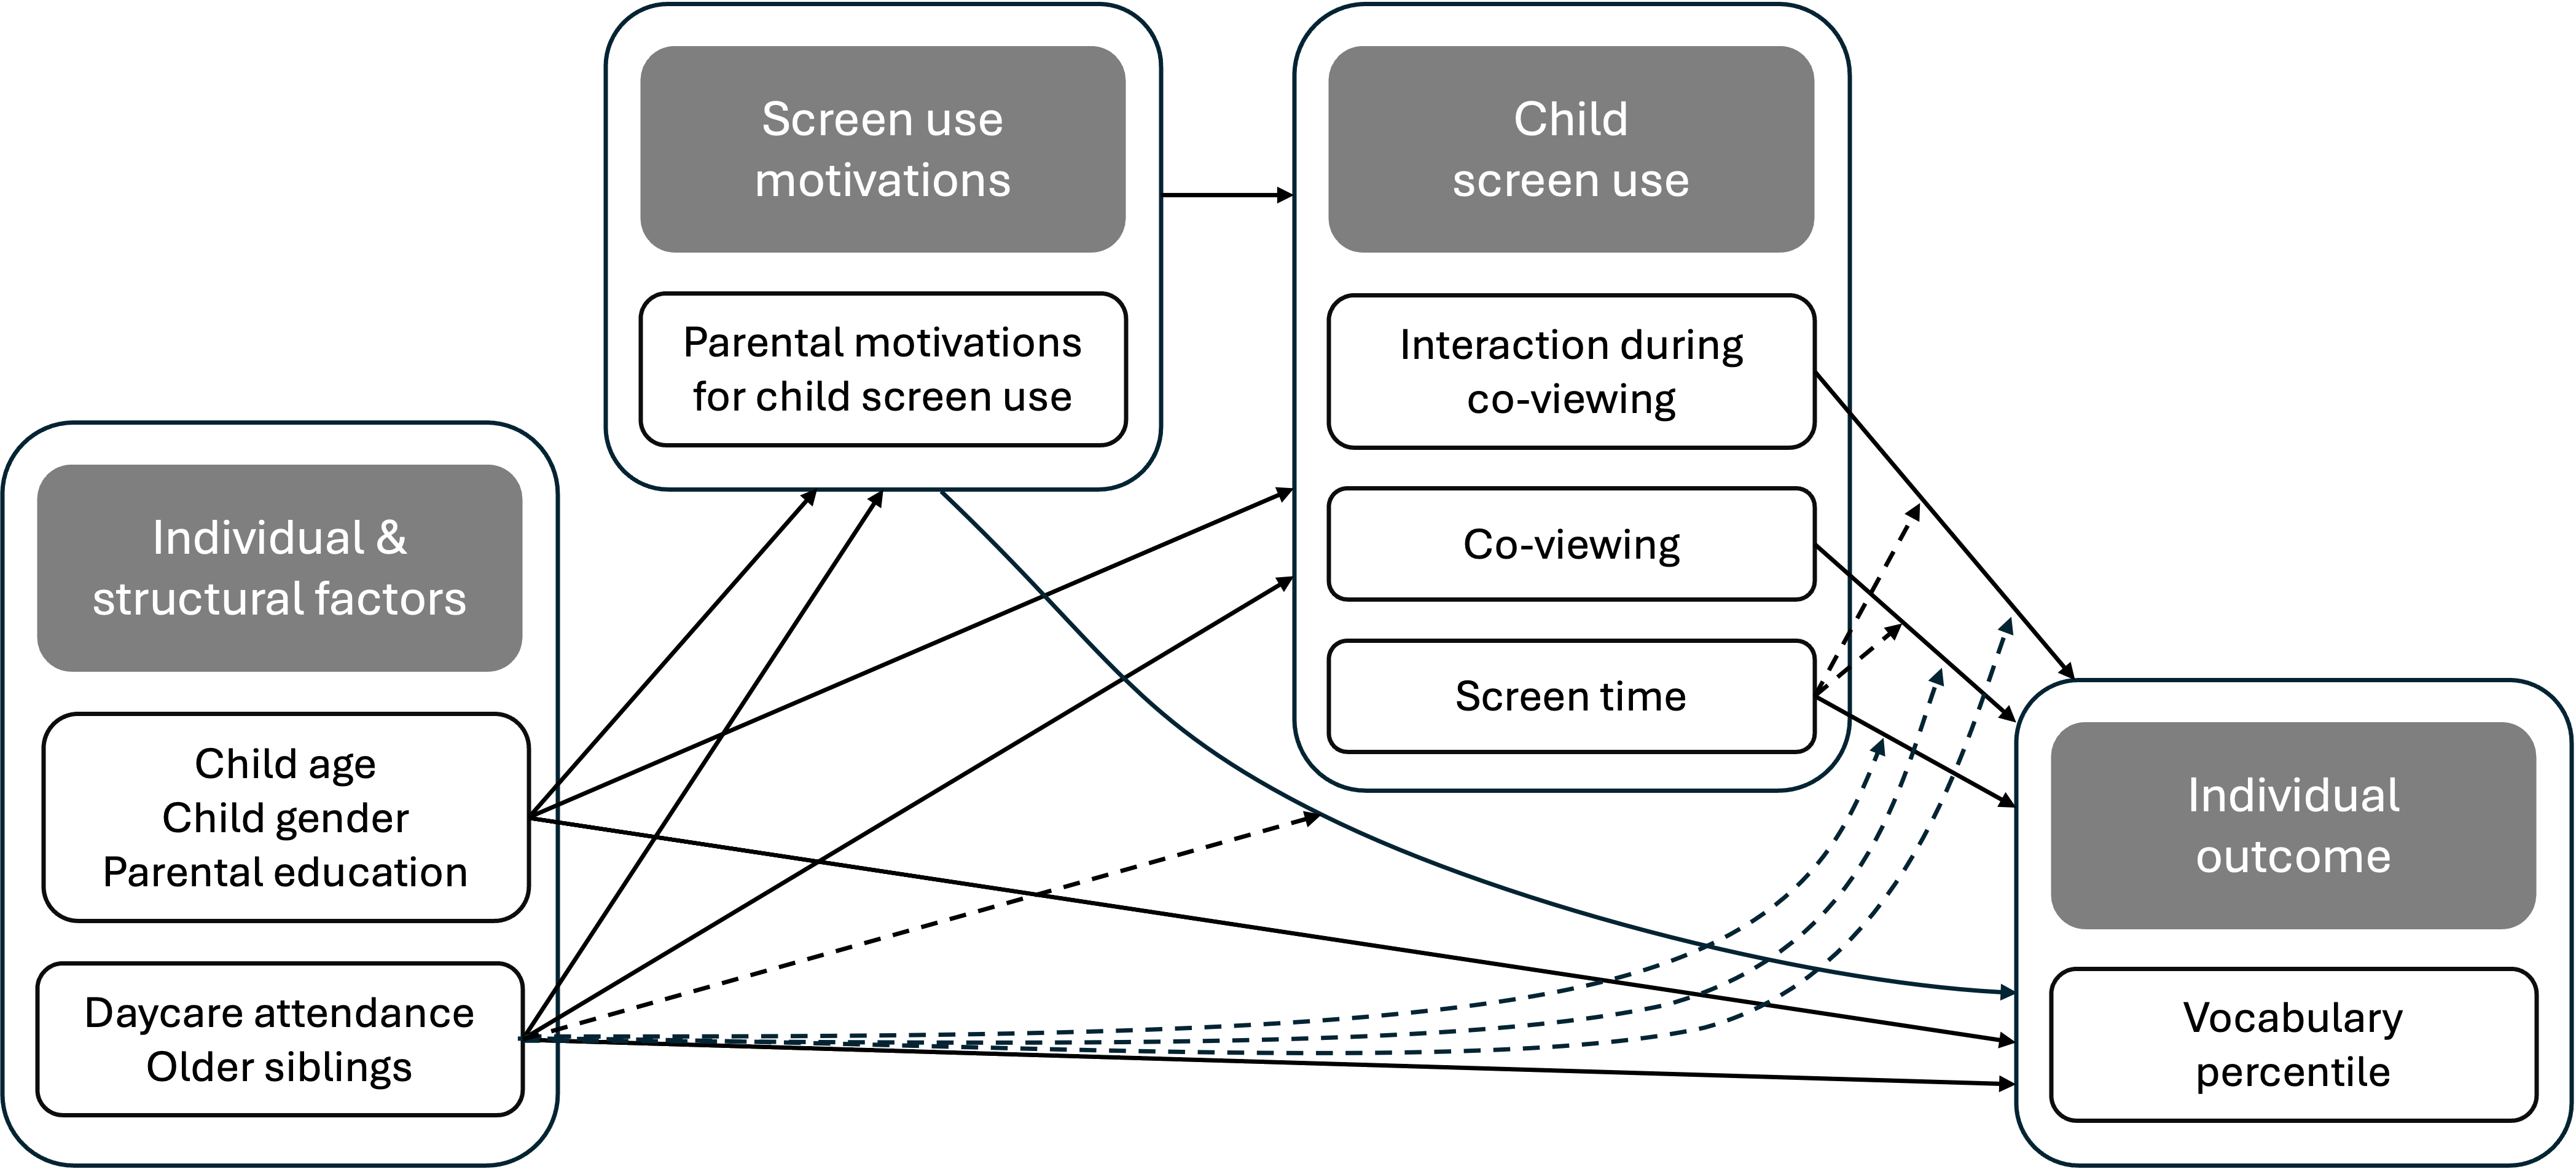
\includegraphics[keepaspectratio]{figs/screenuse_sem.png}}

}

\end{figure}%

\vspace{1em}

\section{Method}\label{method}

\subsection{Sample}\label{sample}

This study was a spin-off of a broader study on child screen use (Swiss
Preschool Screen Exposure, SWIPE;
\citeproc{ref-schmidDigitalMediaUse2025}{Schmid et al., 2025}).
Participants in that study were assigned randomly to one spin-off among
eight possible spin-offs. The sample size for this study was constrained
by the number of participants assigned to this spin-off and by the age
range of the vocabulary assessment tool (8--30 months). Participants
were recruited through a combined offline and online strategy to ensure
broad outreach across all Swiss cantons. Recruitment materials were
available in the three main languages spoken in Switzerland (German,
French, Italian) and English. Offline recruitment included mailing
printed posters and flyers for display in daycare centers, early
childhood organizations, municipalities, midwives, and pediatric
offices. Online recruitment complemented these efforts through targeted
emails and phone calls to daycare directors and early childhood
organizations, as well as outreach via Facebook, Instagram, and blogs.
The goal was to recruit the largest possible sample, to be as
representative as possible in terms of parental educational level, and
to be evenly distributed across the seasons of the year. Given our aim
to collect a large and informative sample for descriptive purposes, we
adopted a flexible data collection approach without a predefined
stopping rule or prior power analysis.

A total of 279 parents of children aged 8--30 months participated in the
present study (see Table~\ref{tbl-demographics} for demographic
information). Inclusion criteria were: (1) having a child aged 8--30
months, (2) parental age between 16--65 years, (3) residing in
Switzerland according to postal code, (4) providing any data on child
digital device present or used, and (5) understanding German, French,
Italian, or English. Exclusion criteria included: (1) not consenting to
participate, (2) giving multiple implausible responses (e.g., partner
age older than 90 years, inappropriate open text answers), or (3)
suspected duplicate participation. For more detailed information on the
study see Schmid and colleagues (citation).

\begingroup
\fontsize{8.2pt}{9.9pt}\selectfont
\setlength{\LTpost}{0mm}

\begin{longtable}[c]{lllll}

\caption{\label{tbl-demographics}Sociodemographic information; values
are expressed as percentages within the geographical location subsample,
unless otherwise specified.}

\tabularnewline



\toprule
 & \multicolumn{4}{c}{Language region in Switzerland} \\ 
\cmidrule(lr){2-5}
Variable & German & French & Italian & Total \\ 
\midrule\addlinespace[2.5pt]
\(N\) & 114 & 130 & 34 & 279 \\ 
\midrule\addlinespace[2.5pt]
\multicolumn{5}{l}{\textbf{Child first language}\textsuperscript{\textit{1}}} \\[2.5pt] 
\midrule\addlinespace[2.5pt]
Swiss German & 86.0 & 3.1 & 2.9 & 36.9 \\ 
German & 18.4 & 3.1 & 0.0 & 9.3 \\ 
French & 11.4 & 96.2 & 2.9 & 49.8 \\ 
Italian & 5.3 & 7.7 & 97.1 & 17.6 \\ 
English & 2.6 & 5.4 & 0.0 & 3.6 \\ 
Other & 6.1 & 9.2 & 0.0 & 6.8 \\ 
\midrule\addlinespace[2.5pt]
\multicolumn{5}{l}{\textbf{Child gender} (\(n=0\) missing)} \\[2.5pt] 
\midrule\addlinespace[2.5pt]
Male/man & 50.9 & 57.7 & 32.4 & 51.6 \\ 
Female/woman & 49.1 & 41.5 & 67.6 & 48.0 \\ 
Diverse\textsuperscript{\textit{2}} & 0.0 & 0.8 & 0.0 & 0.4 \\ 
\midrule\addlinespace[2.5pt]
\multicolumn{5}{l}{\textbf{Child age} (\(n=0\) missing)} \\[2.5pt] 
\midrule\addlinespace[2.5pt]
(mean \(\pm\) SD months) & 24.1 \(\pm\) 4.3 & 21.8 \(\pm\) 6.2 & 20.2 \(\pm\) 6.5 & 22.6 \(\pm\) 5.7 \\ 
\textless{}1 year (\(n = 16\)) & 0.9 & 8.5 & 11.8 & 5.7 \\ 
1--2 years (\(n = 119\)) & 40.4 & 40.8 & 58.8 & 42.7 \\ 
2--3 years (\(n = 144\)) & 58.8 & 50.8 & 29.4 & 51.6 \\ 
\midrule\addlinespace[2.5pt]
\multicolumn{5}{l}{\textbf{Number of siblings}} \\[2.5pt] 
\midrule\addlinespace[2.5pt]
No sibling & 74.6 & 67.7 & 79.4 & 72.0 \\ 
One sibling & 18.4 & 21.5 & 11.8 & 19.0 \\ 
Two siblings & 6.1 & 9.2 & 8.8 & 7.9 \\ 
Three or more siblings & 0.9 & 1.5 & 0.0 & 1.1 \\ 
\midrule\addlinespace[2.5pt]
\multicolumn{5}{l}{\textbf{Parent gender} (\(n=0\) missing)} \\[2.5pt] 
\midrule\addlinespace[2.5pt]
Male/man & 21.1 & 17.7 & 2.9 & 17.2 \\ 
Female/woman & 78.9 & 82.3 & 97.1 & 82.8 \\ 
\midrule\addlinespace[2.5pt]
\multicolumn{5}{l}{\textbf{Parent age} (\(n=0\) missing)} \\[2.5pt] 
\midrule\addlinespace[2.5pt]
(mean \(\pm\) SD months) & 35.1 \(\pm\) 3.8 & 34.7 \(\pm\) 4.6 & 34.0 \(\pm\) 4.6 & 34.8 \(\pm\) 4.3 \\ 
\midrule\addlinespace[2.5pt]
\multicolumn{5}{l}{\textbf{Parent nationality}} \\[2.5pt] 
\midrule\addlinespace[2.5pt]
Non-Swiss & 21.1 & 27.7 & 29.4 & 25.4 \\ 
Swiss & 78.9 & 72.3 & 70.6 & 74.6 \\ 
\midrule\addlinespace[2.5pt]
\multicolumn{5}{l}{\textbf{Parent language}} \\[2.5pt] 
\midrule\addlinespace[2.5pt]
Swiss German & 71.1 & 3.1 & 2.9 & 30.8 \\ 
German & 16.7 & 1.5 & 0.0 & 7.9 \\ 
French & 8.8 & 90.8 & 2.9 & 46.2 \\ 
Italian & 4.4 & 6.2 & 97.1 & 16.5 \\ 
English & 3.5 & 3.8 & 0.0 & 3.2 \\ 
\midrule\addlinespace[2.5pt]
\multicolumn{5}{l}{\textbf{Parental education}} \\[2.5pt] 
\midrule\addlinespace[2.5pt]
Unknown/missing & 0.0 & 0.0 & 0.0 & 0.4 \\ 
Less than primary & 0.0 & 0.8 & 0.0 & 0.4 \\ 
Primary & 2.6 & 0.8 & 2.9 & 1.8 \\ 
Secondary & 8.8 & 13.2 & 38.2 & 14.3 \\ 
Matura degree\textsuperscript{\textit{3}} & 17.5 & 10.9 & 11.8 & 13.6 \\ 
College degree\textsuperscript{\textit{4}} & 25.4 & 26.4 & 23.5 & 25.8 \\ 
Bachelor's degree\textsuperscript{\textit{5}} & 36.8 & 40.3 & 17.6 & 35.8 \\ 
Master's degree\textsuperscript{\textit{6}} & 8.8 & 7.8 & 5.9 & 7.9 \\ 
PhD & 0.0 & 0.0 & 0.0 & 0.0 \\ 
\midrule\addlinespace[2.5pt]
\multicolumn{5}{l}{\textbf{Parent employment category}\textsuperscript{\textit{7}}} \\[2.5pt] 
\midrule\addlinespace[2.5pt]
Not employed & 8.0 & 6.2 & 20.6 & 8.7 \\ 
Unskilled, salesman & 6.2 & 5.4 & 11.8 & 6.9 \\ 
Educator, nurse & 33.0 & 38.5 & 38.2 & 36.1 \\ 
Psychologist, technician & 42.0 & 31.5 & 20.6 & 34.3 \\ 
Senior executive, large business & 10.7 & 18.5 & 8.8 & 14.1 \\ 
\midrule\addlinespace[2.5pt]
\multicolumn{5}{l}{\textbf{Parent work percentage} (\(n=1\) missing)} \\[2.5pt] 
\midrule\addlinespace[2.5pt]
no\% & 4.4 & 2.3 & 17.6 & 5.0 \\ 
0--49\% & 14.0 & 3.9 & 8.8 & 9.0 \\ 
50--100\% & 81.6 & 93.8 & 73.5 & 86.0 \\ 
\midrule\addlinespace[2.5pt]
\multicolumn{5}{l}{\textbf{Perception of financial situation}} \\[2.5pt] 
\midrule\addlinespace[2.5pt]
Far below average & 0.9 & 0.8 & 0.0 & 0.7 \\ 
Somewhat below average & 8.8 & 12.3 & 20.6 & 12.2 \\ 
Average & 29.8 & 33.8 & 55.9 & 34.8 \\ 
Somewhat above average & 52.6 & 43.1 & 20.6 & 44.1 \\ 
Far above average & 7.9 & 8.5 & 2.9 & 7.5 \\ 
Prefer not to say/unknown & 0.0 & 1.5 & 0.0 & 0.7 \\ 
\midrule\addlinespace[2.5pt]
\multicolumn{5}{l}{\textbf{Current partner status} (\(n=0\) missing)} \\[2.5pt] 
\midrule\addlinespace[2.5pt]
Biological parent & 96.5 & 95.4 & 97.1 & 96.1 \\ 
Not biological parent & 0.0 & 2.3 & 0.0 & 1.1 \\ 
No partner & 3.5 & 2.3 & 2.9 & 2.9 \\ 
\bottomrule

\end{longtable}

\hspace*{-\parindent}\begin{minipage}{\linewidth}
\textsuperscript{\textit{1}}Parents selected from the following language options: (Swiss) German, French, Italian, Romansh, and English, with multiple answers possible.\\
\textsuperscript{\textit{2}}Non-binary, third gender, gender-fluid, two-spirit, something else.\\
\textsuperscript{\textit{3}}Baccalaureate schools, Specialized Baccalaureate, Upper secondary specialized schools, Vocational education and training, Vocational education and training (Apprenticeship), FVB, Federal Vet Diploma.\\
\textsuperscript{\textit{4}}College of Higher Education Diploma, Universities of Applied Sciences, Universities of Teacher Education, Universities incl. Federal Institutes of Technology.\\
\textsuperscript{\textit{5}}Bachelor's degree, College of Higher Education Diploma, Federal Diploma of Higher Education.\\
\textsuperscript{\textit{6}}Master's, Advanced Federal Diploma of Higher Education.\\
\textsuperscript{\textit{7}}For employment category examples, see the full survey on OSF (\url{https://osf.io/kd3b7}).\\
\end{minipage}
\endgroup

Among all families, 90\% lived in two-parent households, 2.5\% in
single-parent households, and 12.9\% in other arrangements (unknown:
0.4\%). Child supervision outside the family was reported by 94.6\% of
respondents. These children attended daycare (i.e., childcare service,
64.2\%), kindergarten (i.e., early education, 17.2\%), or were cared for
by a nanny/manny (3.9\%). The mean number of half days of attending
daycare was 5.4 (SD = 2.9, range = {[}0, 14{]}). Other supervision
sources included relatives (39.4\%), day parents (4.3\%), or school
daycare (0.4\%). Regarding health, 2.9\% of children had a physical
illness (e.g., neurodermatitis), and one child (0.4\%) had a
developmental delay (motor delay).

\subsection{Procedure}\label{procedure}

Data were collected through an online survey hosted by Qualtrics XM
(survey available at \url{https://osf.io/kd3b7}). Parents who were
interested in participating in the study accessed the online survey via
a link or QR code displayed on recruitment materials. Data were
collected between February 1, 2023, and May 31, 2024. A welcome page
provided the aims of the study, explained what participation in the
study consisted of, that the study could be completed anonymously, and
gave contact information of the study personnel. Parental informed
consent was requested to proceed to the survey. The first part of the
survey consisted of a core questionnaire that collected demographic
information and child digital media (DM) usage for all participants. The
second part consisted of eight spin-offs, one of which was focused on
assessing language skills in young children. Parents from the current
study have been randomly assigned to the language spinoff. Completion of
the survey took about 30-45 minutes.

The study was approved by the Cantonal Ethics Committee Zurich,
Switzerland (statement of non-responsibility). Participants were offered
to sign up for a lottery to win one of 30 $\times$ CHF 100 gift vouchers using
a second form hosted on an independent Qualtrics XM account.

\subsection{Measures}\label{measures}

The core questionnaire, adapted from the broader SWIPE study
(\citeproc{ref-schmidDigitalMediaUse2025}{Schmid et al., 2025}),
comprised 48 items across two main sections: demographic information and
child DM use. The demographic section included detailed questions about
the responding parent, the child's other parent, household structure,
and child characteristics (e.g., age, gender, health, supervision, and
language background). The DM section assessed four key dimensions:
device accessibility, usage duration, content characteristics, and usage
context.

Device accessibility was measured by asking parents which digital
devices were present in the household and whether their child had used
them. For usage duration, parents estimated average daily time spent on
various DM activities (e.g., video watching, app use, audio listening)
across weekdays and weekends, with implausible values excluded during
preprocessing. Content characteristics were rated using Likert scales
and included dimensions such as educational value, emotional themes,
prosocial behavior, and language exposure. Contextual factors included
parental motivations for screen use, co-viewing behaviors, and the
timing of media use throughout the day. Notably, the questionnaire
captured general caregiver perceptions rather than context-specific
(e.g., home vs.~daycare) media use. For a comprehensive description of
the survey design and item development, see Schmid and colleagues
(\citeproc{ref-schmidDigitalMediaUse2025}{2025}).

Language abilities of children were assessed with the full version of
the MacArthur-Bates Communicative Development Inventory (CDI;
\citeproc{ref-fensonMacArthurBatesCommunicativeDevelopment2007}{Fenson
et al., 2007}), which was available to the study participants in either
German, French, Italian, or English depending on the preferred language
by the parent. The CDI is a standardized parent-report questionnaire
designed to assess early language development in infants and toddlers.
Depending on the version used (e.g., Words and Gestures for children
aged 8--18 months or Words and Sentences for children aged 16--30
months), it captures vocabulary comprehension and production, gesture
use, and early grammatical abilities. Parents completed the inventory by
indicating which words or gestures their child understands and/or
produces, offering a reliable and developmentally sensitive measure of
communicative milestones in the 8- to 30-month age range. Based on the
vocabulary items, the CDI allows one to generate a total vocabulary
score that was converted to a percentile score depending on the child's
age (see next section).

\subsection{Data analysis}\label{data-analysis}

To analyze the data, we first prepared the data by conducting factor
analysis on our screen use variables and converting CDI scores to
percentiles, and then we conducted Bayesian causal mediation analysis
with CDI percentiles as the outcome.

\subsubsection{Data preprocessing}\label{data-preprocessing}

To prepare the data for analysis, we first conducted exploratory factor
analysis on parental motivations for child screen use, and parent--child
interactions during co-viewing of screens. For both groups, we used
parallel analysis (\citeproc{ref-hornRationaleTestNumber1965}{Horn,
1965}) to determine the number of factors to extract. We used the
\texttt{psych} package
(\citeproc{ref-revellePsychProceduresPsychological2025}{Revelle, 2025})
to perform factor analysis on each group separately with varimax
rotation, using the latent factor scores as variables in our analysis.

To convert the CDI vocabulary scores to percentiles, we obtained data
for the relevant CDI instruments from Wordbank
(\citeproc{ref-frankWordbankOpenRepository2017}{Frank et al., 2017}),
accessed using the \texttt{wordbankr} package
(\citeproc{ref-braginskyWordbankrAccessingWordbank2022}{Braginsky,
2022}). We included all data from monolinguals, using expressive
vocabulary scores for Words \& Sentences forms (16--30 months) and
receptive vocabulary scores for Words \& Gestures forms (8--16 months);
these scores were converted into proportions of the maximum score for
each form. Following previous work
(\citeproc{ref-marchmanMacArthurBatesCommunicativeDevelopment2023}{Marchman
et al., 2023}), we then fit the vocabulary proportions using generalised
additive models for location, shape, and scale (GAMLSS;
\citeproc{ref-stasinopoulosFlexibleRegressionSmoothing2017}{Stasinopoulos
et al., 2017}) with a beta distribution, using the \texttt{gamlss}
package
(\citeproc{ref-stasinopoulosGamlssGeneralizedAdditive2024}{Stasinopoulos
et al., 2024}). The models included monotonic P-splines for age for both
location and scale, with a smoothing parameter of 10000. We also
included random effects for child when there were longitudinal data
(i.e., children who contributed to Wordbank at multiple time points).
The fitted models were used to estimate vocabulary percentiles for each
child, which we used as the outcome variable in our analysis. Four
parents filled in CDIs in two languages for their children (indicating
that they considered their child to have two first languages); we
averaged the vocabulary percentiles for these children.

We also preprocessed our other predictor variables. Age was
mean-centered. Gender was treated as a binary variable with sum
contrasts (male \(= - 0.5\), female \(= 0.5\)). Parental education was
treated as an ordinal variable with polynomial contrasts. Whether
children were accompanied during screen use (i.e., co-viewing) was
treated as a binary variable.

\subsubsection{Causal mediation
analysis}\label{causal-mediation-analysis}

To test the validity of the DREAMER framework in this study, we
conducted a causal serial mediation analysis using the potential
outcomes framework (\citeproc{ref-imaiGeneralApproachCausal2010}{Imai et
al., 2010}; \citeproc{ref-valeriMediationAnalysisAllowing2013}{Valeri \&
VanderWeele, 2013}). We used the \texttt{blavaan} package
(\citeproc{ref-merkleBlavaanBayesianStructural2018}{Merkle \& Rosseel,
2018}) to fit a Bayesian structural equation model (SEM) to the data.
The SEM was specified with five groups of variables: (1)
individual-level covariates (age, gender, parental education); (2)
structural factors (number of half days per week the child attends
daycare, number of older siblings); (3) first-level mediators (parental
motivations for child screen use); (4) second-level mediators
(children's weekly screen time, whether children use screens while
accompanied, parental interaction during screen co-viewing); and (5)
outcome (vocabulary percentiles).

In the first step of the model, the first-level mediators were predicted
by the individual-level covariates and structural factors. In the second
step, the second-level mediators were predicted by the first-level
mediators, individual-level covariates, and structural factors. Finally,
in the third step, the outcome was predicted by the second-level
mediators, first-level mediators, individual-level covariates, and
structural factors, as well as interactions between the structural
factors and all mediators, and between screen time and all other
second-level mediators. A schematic path diagram of the model is shown
in Figure 1.

For both structural factors (amount of half days of daycare and number
of older siblings), we also calculated the pure natural direct effects
(PNDEs), total natural direct effects (TNDEs), pure natural indirect
effects (PNIEs), total natural indirect effects (TNIEs), and total
effects (TEs).\footnote{The PNDE is the direct effect of the predictor
  on the outcome if the mediator were held at its control value. The
  TNDE is the direct effect of the predictor on the outcome if the
  mediator were held at its treatment value. The PNIE is the indirect
  effect of the predictor on the outcome via the mediator, if the
  predictor were held at its control value. The TNIE is the indirect
  effect of the predictor on the outcome via the mediator, if the
  predictor were held at its treatment value. The total effect is the
  overall effect of the predictor on the outcome, and is equal to PNDE +
  TNIE or TNDE + PNIE.} For the amount of half days in daycare, the
effects were calculated for one additional half day of daycare per week,
and for the number of older siblings, the effects were calculated for
one additional older sibling. Reference values for the covariates were
the mean age, the zero value for sum-contrasted gender, and the modal
value for parental education (corresponding to a bachelor's degree).

We used weakly informative priors for all parameters: normal priors with
mean 0 and standard deviation 10 for all coefficients and intercepts, LKJ
priors with uniform density for all covariances, and gamma priors with
alpha 1 and beta 0.5 for all variances. We used 4 chains of 8000
iterations each, with the first 1000 iterations discarded as burn-in.
Missing data were treated as missing at random; our model employed full
information likelihood for estimation.

\vspace{1em}

\section{Results}\label{results}

We first report the results of the factor analyses of our mediators,
followed by the overall effects of the structural factors on CDI
percentiles in our causal mediation analysis. We then investigate the
components of our causal mediation analysis to further understand the
relationship among our variables of interest.

\subsection{Factor analyses}\label{factor-analyses}

For parental motivations for letting children use screens, parallel
analysis suggested a four-factor solution. Factor loadings for each of
the parental motivation items are shown in
Table~\ref{tbl-fa-motivation}. The first factor is related to child
behavioral management, involving items relating to modifying the child's
behavior. The second factor is related to occupying the child so as to
free up time for the parent to do other tasks or to reduce parents'
stress. The third factor is related to screen use as a means of
learning, whether it be learning facts, languages, or about the digital
world itself. The fourth factor is related to emotion regulation of the
child, including items relating to calming the child down and reducing
their anger.

\begin{table}

{\caption{{Loadings from the factor analysis of the parental screen use
motivation items, showing a four-factor
solution.}{\label{tbl-fa-motivation}}}}

\fontsize{8.2pt}{9.9pt}\selectfont
\begin{tabular*}{\linewidth}{@{\extracolsep{\fill}}>{\raggedright\arraybackslash}p{\dimexpr 187.50pt -2\tabcolsep-1.5\arrayrulewidth}>{\raggedleft\arraybackslash}p{\dimexpr 67.50pt -2\tabcolsep-1.5\arrayrulewidth}>{\raggedleft\arraybackslash}p{\dimexpr 67.50pt -2\tabcolsep-1.5\arrayrulewidth}>{\raggedleft\arraybackslash}p{\dimexpr 67.50pt -2\tabcolsep-1.5\arrayrulewidth}>{\raggedleft\arraybackslash}p{\dimexpr 67.50pt -2\tabcolsep-1.5\arrayrulewidth}}
\toprule
 & \multicolumn{4}{>{\centering\arraybackslash}m{\dimexpr 270.00pt -2\tabcolsep-1.5\arrayrulewidth}}{Factor loadings} \\ 
\cmidrule(lr){2-5}
Item & Behavioral management & Freeing parent & Learning & Emotion regulation \\ 
\midrule\addlinespace[2.5pt]
The reason for screen use is to make him/her sleepy & {\cellcolor[HTML]{3178B5}{\textcolor[HTML]{FFFFFF}{0.72}}} & {\cellcolor[HTML]{E2EDF3}{\textcolor[HTML]{000000}{0.11}}} & {\cellcolor[HTML]{F6F6F7}{\textcolor[HTML]{000000}{0.01}}} & {\cellcolor[HTML]{D4E6F1}{\textcolor[HTML]{000000}{0.18}}} \\ 
The reason for screen use is to regulate his/her boredom & {\cellcolor[HTML]{529BC7}{\textcolor[HTML]{FFFFFF}{0.57}}} & {\cellcolor[HTML]{D9E9F1}{\textcolor[HTML]{000000}{0.16}}} & {\cellcolor[HTML]{CBE2EE}{\textcolor[HTML]{000000}{0.22}}} & {\cellcolor[HTML]{DCEAF2}{\textcolor[HTML]{000000}{0.14}}} \\ 
The reason for screen use is to help him/her eat better & {\cellcolor[HTML]{68A8CE}{\textcolor[HTML]{FFFFFF}{0.52}}} & {\cellcolor[HTML]{E6EFF4}{\textcolor[HTML]{000000}{0.09}}} & {\cellcolor[HTML]{DDEBF2}{\textcolor[HTML]{000000}{0.14}}} & {\cellcolor[HTML]{E1ECF3}{\textcolor[HTML]{000000}{0.12}}} \\ 
The reason for screen use is to spend time with my friends, family, or partner (e.g., to have a quiet meal) & {\cellcolor[HTML]{71AED2}{\textcolor[HTML]{000000}{0.49}}} & {\cellcolor[HTML]{E6EFF4}{\textcolor[HTML]{000000}{0.09}}} & {\cellcolor[HTML]{DBEAF2}{\textcolor[HTML]{000000}{0.15}}} & {\cellcolor[HTML]{ABD1E5}{\textcolor[HTML]{000000}{0.32}}} \\ 
The reason for screen use is to get my housework done & {\cellcolor[HTML]{DCEAF2}{\textcolor[HTML]{000000}{0.14}}} & {\cellcolor[HTML]{357EB8}{\textcolor[HTML]{FFFFFF}{0.69}}} & {\cellcolor[HTML]{D0E4F0}{\textcolor[HTML]{000000}{0.20}}} & {\cellcolor[HTML]{EFF3F6}{\textcolor[HTML]{000000}{0.04}}} \\ 
The reason for screen use is to get work done & {\cellcolor[HTML]{4A97C5}{\textcolor[HTML]{FFFFFF}{0.58}}} & {\cellcolor[HTML]{3984BB}{\textcolor[HTML]{FFFFFF}{0.67}}} & {\cellcolor[HTML]{E5EFF4}{\textcolor[HTML]{000000}{0.09}}} & {\cellcolor[HTML]{FAEDE5}{\textcolor[HTML]{000000}{-0.07}}} \\ 
The reason for screen use is to calm myself down, when I am stressed & {\cellcolor[HTML]{E6EFF4}{\textcolor[HTML]{000000}{0.09}}} & {\cellcolor[HTML]{3B87BD}{\textcolor[HTML]{FFFFFF}{0.65}}} & {\cellcolor[HTML]{C0DCEB}{\textcolor[HTML]{000000}{0.26}}} & {\cellcolor[HTML]{A3CDE3}{\textcolor[HTML]{000000}{0.35}}} \\ 
The reason for screen use is to have some peace for myself & {\cellcolor[HTML]{DCEAF2}{\textcolor[HTML]{000000}{0.14}}} & {\cellcolor[HTML]{66A6CE}{\textcolor[HTML]{FFFFFF}{0.52}}} & {\cellcolor[HTML]{B0D4E6}{\textcolor[HTML]{000000}{0.31}}} & {\cellcolor[HTML]{A0CCE2}{\textcolor[HTML]{000000}{0.36}}} \\ 
The reason for screen use is to learn something new & {\cellcolor[HTML]{D2E6F0}{\textcolor[HTML]{000000}{0.19}}} & {\cellcolor[HTML]{E2EDF3}{\textcolor[HTML]{000000}{0.11}}} & {\cellcolor[HTML]{2065AA}{\textcolor[HTML]{FFFFFF}{0.80}}} & {\cellcolor[HTML]{FBEAE0}{\textcolor[HTML]{000000}{-0.10}}} \\ 
The reason for screen use is to improve his/her native language & {\cellcolor[HTML]{C6DFED}{\textcolor[HTML]{000000}{0.24}}} & {\cellcolor[HTML]{D5E7F1}{\textcolor[HTML]{000000}{0.18}}} & {\cellcolor[HTML]{519AC7}{\textcolor[HTML]{FFFFFF}{0.57}}} & {\cellcolor[HTML]{F8F2EF}{\textcolor[HTML]{000000}{-0.03}}} \\ 
The reason for screen use is to learn a foreign language & {\cellcolor[HTML]{DEEBF2}{\textcolor[HTML]{000000}{0.13}}} & {\cellcolor[HTML]{D6E7F1}{\textcolor[HTML]{000000}{0.17}}} & {\cellcolor[HTML]{5FA3CC}{\textcolor[HTML]{FFFFFF}{0.54}}} & {\cellcolor[HTML]{E7EFF4}{\textcolor[HTML]{000000}{0.09}}} \\ 
The reason for screen use is to be prepared for the digital future & {\cellcolor[HTML]{F9EFEA}{\textcolor[HTML]{000000}{-0.05}}} & {\cellcolor[HTML]{E3EDF3}{\textcolor[HTML]{000000}{0.11}}} & {\cellcolor[HTML]{7EB7D6}{\textcolor[HTML]{000000}{0.46}}} & {\cellcolor[HTML]{D6E7F1}{\textcolor[HTML]{000000}{0.18}}} \\ 
The reason for screen use is to calm him/her down & {\cellcolor[HTML]{A1CCE2}{\textcolor[HTML]{000000}{0.35}}} & {\cellcolor[HTML]{CAE1EE}{\textcolor[HTML]{000000}{0.22}}} & {\cellcolor[HTML]{D5E7F1}{\textcolor[HTML]{000000}{0.18}}} & {\cellcolor[HTML]{6FADD1}{\textcolor[HTML]{000000}{0.50}}} \\ 
The reason for screen use is to help him/her to not be angry anymore & {\cellcolor[HTML]{C8E0ED}{\textcolor[HTML]{000000}{0.23}}} & {\cellcolor[HTML]{EAF1F5}{\textcolor[HTML]{000000}{0.07}}} & {\cellcolor[HTML]{F9F0EA}{\textcolor[HTML]{000000}{-0.05}}} & {\cellcolor[HTML]{84BBD9}{\textcolor[HTML]{000000}{0.44}}} \\ 
\bottomrule
\end{tabular*}

\end{table}

For parental interactions during screen co-viewing, parallel analysis
suggested a three-factor solution. Factor loadings for each of the
parental interaction items are shown in Table~\ref{tbl-fa-interaction}.
The first factor is related to the parent drawing in other information
by expanding on content, reinforcing ideas, or relating content to other
ideas. The second factor is related to the parent focusing the child's
attention on the content by commenting, naming, or pointing to aspects
of the content. The third factor is related to the parent asking
questions about the content, including asking about what is happening or
asking the child to name aspects of the content.

\begin{table}

{\caption{{Loadings from the factor analysis of the items on
parent--child interaction during screen use, showing a three-factor
solution.}{\label{tbl-fa-interaction}}}}

\fontsize{8.2pt}{9.9pt}\selectfont
\begin{tabular*}{\linewidth}{@{\extracolsep{\fill}}>{\raggedright\arraybackslash}p{\dimexpr 255.00pt -2\tabcolsep-1.5\arrayrulewidth}>{\raggedleft\arraybackslash}p{\dimexpr 67.50pt -2\tabcolsep-1.5\arrayrulewidth}>{\raggedleft\arraybackslash}p{\dimexpr 67.50pt -2\tabcolsep-1.5\arrayrulewidth}>{\raggedleft\arraybackslash}p{\dimexpr 67.50pt -2\tabcolsep-1.5\arrayrulewidth}}
\toprule
 & \multicolumn{3}{>{\centering\arraybackslash}m{\dimexpr 202.50pt -2\tabcolsep-1.5\arrayrulewidth}}{Factor loadings} \\ 
\cmidrule(lr){2-4}
Item & Expanding & Focusing & Asking \\ 
\midrule\addlinespace[2.5pt]
Expand on what he/she says (e.g., rephrase, add information to what your child was saying) & {\cellcolor[HTML]{2E74B3}{\textcolor[HTML]{FFFFFF}{0.74}}} & {\cellcolor[HTML]{A6CFE4}{\textcolor[HTML]{000000}{0.34}}} & {\cellcolor[HTML]{D2E5F0}{\textcolor[HTML]{000000}{0.20}}} \\ 
Reinforce the understanding of what is happening (e.g., who is that? where do they live? Why are they doing what they're doing?) & {\cellcolor[HTML]{3178B5}{\textcolor[HTML]{FFFFFF}{0.72}}} & {\cellcolor[HTML]{C3DEEC}{\textcolor[HTML]{000000}{0.24}}} & {\cellcolor[HTML]{BBD9E9}{\textcolor[HTML]{000000}{0.27}}} \\ 
Relate the content to what your child feels or thinks & {\cellcolor[HTML]{3F8CC0}{\textcolor[HTML]{FFFFFF}{0.63}}} & {\cellcolor[HTML]{D8E8F1}{\textcolor[HTML]{000000}{0.16}}} & {\cellcolor[HTML]{D7E8F1}{\textcolor[HTML]{000000}{0.17}}} \\ 
Pause the program to explain something & {\cellcolor[HTML]{BCDAEA}{\textcolor[HTML]{000000}{0.27}}} & {\cellcolor[HTML]{D9E9F1}{\textcolor[HTML]{000000}{0.16}}} & {\cellcolor[HTML]{BDDAEA}{\textcolor[HTML]{000000}{0.27}}} \\ 
Comment on what's on the screen & {\cellcolor[HTML]{CCE3EF}{\textcolor[HTML]{000000}{0.22}}} & {\cellcolor[HTML]{2C72B2}{\textcolor[HTML]{FFFFFF}{0.75}}} & {\cellcolor[HTML]{D8E8F1}{\textcolor[HTML]{000000}{0.16}}} \\ 
Name what's on the screen & {\cellcolor[HTML]{D7E8F1}{\textcolor[HTML]{000000}{0.17}}} & {\cellcolor[HTML]{3780BA}{\textcolor[HTML]{FFFFFF}{0.68}}} & {\cellcolor[HTML]{BBDAEA}{\textcolor[HTML]{000000}{0.27}}} \\ 
Point to items that are on the screen & {\cellcolor[HTML]{ADD2E5}{\textcolor[HTML]{000000}{0.32}}} & {\cellcolor[HTML]{3E8BBF}{\textcolor[HTML]{FFFFFF}{0.64}}} & {\cellcolor[HTML]{E5EFF4}{\textcolor[HTML]{000000}{0.09}}} \\ 
Ask him/her about what happens in the content watched on the screen & {\cellcolor[HTML]{BAD9E9}{\textcolor[HTML]{000000}{0.27}}} & {\cellcolor[HTML]{CEE3EF}{\textcolor[HTML]{000000}{0.21}}} & {\cellcolor[HTML]{0E4178}{\textcolor[HTML]{FFFFFF}{0.94}}} \\ 
Ask him/her to name the things that are shown on the screen & {\cellcolor[HTML]{9ECBE1}{\textcolor[HTML]{000000}{0.36}}} & {\cellcolor[HTML]{84BBD9}{\textcolor[HTML]{000000}{0.44}}} & {\cellcolor[HTML]{7FB7D7}{\textcolor[HTML]{000000}{0.45}}} \\ 
\bottomrule
\end{tabular*}

\end{table}

\subsection{Causal mediation
analysis}\label{causal-mediation-analysis-1}

The causal mediation SEM converged with all \(\hat{R} <\) 1.011, and
effective sample sizes above 1000. For all estimates, we report the
posterior mean and 95\% highest density credible intervals (CrIs);
reliability was determined by whether the CrI included zero. Descriptive
statistics for all variables included in the model are displayed in
Table~\ref{tbl-supp}.

The overall effects of the structural factors on vocabulary percentiles
are shown in Table~\ref{tbl-overall-effects}. The CrI for the total
effect of the amount of half days of daycare on vocabulary percentiles
included zero, as did all direct and indirect effects. Similarly, the
CrI for the total effect of the number of older siblings on vocabulary
percentiles included zero, as did all direct and indirect effects. These
results suggest that neither the number of half days the child attends
daycare, nor the number of older siblings had a reliable effect on
vocabulary percentiles in this sample.

\begin{table}

{\caption{{Overall effects of structural factors on vocabulary
percentiles, showing posterior means and 95\% highest density credible
intervals. All estimates are for one additional half day of daycare per
week or one additional older sibling.}{\label{tbl-overall-effects}}}}

\fontsize{12.0pt}{14.4pt}\selectfont
\begin{tabular*}{\linewidth}{@{\extracolsep{\fill}}lcc}
\toprule
Effect & Number of half days of daycare & Number of older siblings \\ 
\midrule\addlinespace[2.5pt]
PNDE & 3.14 {[}-0.62, 6.77{]} & -0.35 {[}-16.76, 15.62{]} \\ 
TNDE & 3.12 {[}-0.49, 6.75{]} & -0.28 {[}-16.54, 16.71{]} \\ 
PNIE & -0.71 {[}-1.96, 0.44{]} & 0.23 {[}-3.82, 4.58{]} \\ 
TNIE & -0.73 {[}-1.87, 0.39{]} & 0.30 {[}-5.92, 6.59{]} \\ 
TE & 2.41 {[}-1.14, 6.21{]} & -0.05 {[}-16.75, 17.08{]} \\ 
\bottomrule
\end{tabular*}

\end{table}

\subsection{Component effects}\label{component-effects}

To further understand the model, we examined its individual steps,
considering the predictors of the first-level mediators, the
second-level mediators, and the outcome.

\subsubsection{First-level mediators}\label{first-level-mediators}

Predictors of the first-level mediators are shown in
Table~\ref{tbl-first-level-med}. Both the parental motivations of
behavioral management and freeing up parents had parental education
effects; these effects are visualised in
Figure~\ref{fig-first-level-ses}, suggesting that parents with the
lowest education levels experienced greater motivations for freeing up
time, along with a more complex nonlinear effect for behavioral
management. There was also an effect of child gender, such that parents
of girls were more likely to employ child screen use to free themselves
up. The learning motivation had a reliable effect of age, such that
children who were one year older also had parents who were more
motivated to use screens for learning. All other predictors of the
first-level mediators had CrIs that included zero, suggesting no
reliable effects.

\begin{table}

{\caption{{Predictors of first-level mediators, showing posterior means
and 95\% highest density credible intervals. All estimates are on the
original scale of the mediator. Bolded values indicate reliable
effects.}{\label{tbl-first-level-med}}}}

\fontsize{8.2pt}{9.9pt}\selectfont
\begin{tabular*}{\linewidth}{@{\extracolsep{\fill}}>{\raggedright\arraybackslash}p{\dimexpr 120.00pt -2\tabcolsep-1.5\arrayrulewidth}>{\centering\arraybackslash}p{\dimexpr 82.50pt -2\tabcolsep-1.5\arrayrulewidth}>{\centering\arraybackslash}p{\dimexpr 82.50pt -2\tabcolsep-1.5\arrayrulewidth}>{\centering\arraybackslash}p{\dimexpr 82.50pt -2\tabcolsep-1.5\arrayrulewidth}>{\centering\arraybackslash}p{\dimexpr 82.50pt -2\tabcolsep-1.5\arrayrulewidth}}
\toprule
 & \multicolumn{4}{>{\centering\arraybackslash}m{\dimexpr 330.00pt -2\tabcolsep-1.5\arrayrulewidth}}{Motivation} \\ 
\cmidrule(lr){2-5}
Predictor & Behavioral management & Freeing parent & Learning & Emotion regulation \\ 
\midrule\addlinespace[2.5pt]
Intercept & -0.12 {[}-0.32, 0.09{]} & 0.11 {[}-0.13, 0.36{]} & -0.18 {[}-0.44, 0.06{]} & 0.02 {[}-0.20, 0.25{]} \\ 
Child age & 0.00 {[}-0.01, 0.02{]} & 0.02 {[}0.00, 0.04{]} & \textbf{0.04 {[}0.02, 0.06{]}} & -0.01 {[}-0.03, 0.01{]} \\ 
Child gender & 0.18 {[}0.00, 0.35{]} & \textbf{0.22 {[}0.00, 0.44{]}} & 0.10 {[}-0.12, 0.32{]} & 0.07 {[}-0.13, 0.27{]} \\ 
Parental education: Linear & \textbf{3.24 {[}1.24, 5.20{]}} & \textbf{-2.84 {[}-5.13, -0.51{]}} & -0.88 {[}-3.14, 1.32{]} & -0.93 {[}-3.00, 1.17{]} \\ 
Parental education: Quadratic & \textbf{-6.34 {[}-9.04, -3.63{]}} & 2.75 {[}-0.41, 5.82{]} & 0.64 {[}-2.32, 3.66{]} & 0.25 {[}-2.55, 3.04{]} \\ 
Parental education: Cubic & \textbf{10.14 {[}6.70, 13.29{]}} & -1.30 {[}-5.12, 2.51{]} & 0.92 {[}-2.68, 4.58{]} & -1.04 {[}-4.45, 2.36{]} \\ 
Parental education: Quartic & \textbf{-9.93 {[}-12.51, -7.34{]}} & 1.79 {[}-1.25, 4.73{]} & -1.12 {[}-4.00, 1.69{]} & -0.79 {[}-3.46, 1.80{]} \\ 
Parental education: Quintic & \textbf{8.20 {[}6.21, 10.39{]}} & 1.99 {[}-0.40, 4.56{]} & 1.47 {[}-0.92, 3.88{]} & 1.24 {[}-0.91, 3.46{]} \\ 
Number of half days of daycare & 0.00 {[}-0.03, 0.03{]} & -0.02 {[}-0.06, 0.02{]} & 0.03 {[}-0.01, 0.07{]} & -0.01 {[}-0.04, 0.03{]} \\ 
Nummber of older siblings & 0.16 {[}-0.02, 0.34{]} & -0.06 {[}-0.27, 0.14{]} & -0.08 {[}-0.29, 0.13{]} & -0.02 {[}-0.21, 0.16{]} \\ 
\bottomrule
\end{tabular*}

\end{table}

\begin{figure}

\caption{\label{fig-first-level-ses}Estimated effects of parental
education on first-level mediators, showing posterior means and 95\%
highest density credible intervals. All estimates are on the original
scale of the mediator.}

\centering{

\pandocbounded{\includegraphics[keepaspectratio]{screenuse-vocab_files/figure-pdf/fig-first-level-ses-1.pdf}}

}

\end{figure}%

\subsubsection{Second-level mediators}\label{second-level-mediators}

Predictors of the second-level mediators are shown in
Table~\ref{tbl-second-level-med}. For expanding parental interaction
during co-viewing, the effect of age was reliable and positive, such
that parents of older children were more likely to expand on the content
on the screen. For the focusing interaction, the reliable effects were
of gender and learning motivation, such that parents of boys and parents
who were more motivated by their child's learning were more likely to
focus the child's attention on the content during co-viewing. For the
asking interaction, the effect of age was reliable and positive, such
that parents of older children were more likely to ask about content on
the screen.

\begin{table}

{\caption{{Predictors of second-level mediators, showing posterior means
and 95\% highest density credible intervals. All estimates are on the
original scale of the mediator except for co-viewing, which is on the
logit scale. Bolded values indicate reliable
effects.}{\label{tbl-second-level-med}}}}

\fontsize{8.2pt}{9.9pt}\selectfont
\begin{tabular*}{\linewidth}{@{\extracolsep{\fill}}>{\raggedright\arraybackslash}p{\dimexpr 112.50pt -2\tabcolsep-1.5\arrayrulewidth}>{\centering\arraybackslash}p{\dimexpr 67.50pt -2\tabcolsep-1.5\arrayrulewidth}>{\centering\arraybackslash}p{\dimexpr 67.50pt -2\tabcolsep-1.5\arrayrulewidth}>{\centering\arraybackslash}p{\dimexpr 67.50pt -2\tabcolsep-1.5\arrayrulewidth}>{\centering\arraybackslash}p{\dimexpr 67.50pt -2\tabcolsep-1.5\arrayrulewidth}>{\centering\arraybackslash}p{\dimexpr 67.50pt -2\tabcolsep-1.5\arrayrulewidth}}
\toprule
 & \multicolumn{3}{>{\centering\arraybackslash}m{\dimexpr 202.50pt -2\tabcolsep-1.5\arrayrulewidth}}{Interaction} &  &  \\ 
\cmidrule(lr){2-4}
Predictor & Expanding & Focusing & Asking & Co-viewing & Weekly screen time \\ 
\midrule\addlinespace[2.5pt]
Intercept & 0.10 {[}-0.13, 0.35{]} & -0.19 {[}-0.42, 0.05{]} & -0.19 {[}-0.47, 0.09{]} & -1.31 {[}-2.00, -0.65{]} & 5.49 {[}3.91, 7.08{]} \\ 
Child age & \textbf{0.03 {[}0.01, 0.05{]}} & 0.02 {[}0.00, 0.04{]} & \textbf{0.03 {[}0.01, 0.05{]}} & \textbf{0.12 {[}0.07, 0.17{]}} & \textbf{0.15 {[}0.01, 0.27{]}} \\ 
Child gender & 0.09 {[}-0.12, 0.31{]} & \textbf{-0.29 {[}-0.50, -0.08{]}} & -0.02 {[}-0.27, 0.23{]} & -0.21 {[}-0.78, 0.34{]} & -0.43 {[}-1.85, 1.01{]} \\ 
Parental education: Linear & 0.07 {[}-2.04, 2.10{]} & 1.83 {[}-0.13, 3.85{]} & -1.77 {[}-4.20, 0.51{]} & -1.78 {[}-7.40, 3.70{]} & -7.42 {[}-18.69, 4.02{]} \\ 
Parental education: Quadratic & 0.57 {[}-1.71, 2.74{]} & 0.19 {[}-2.01, 2.30{]} & 1.08 {[}-1.52, 3.62{]} & -1.07 {[}-6.57, 4.75{]} & 10.51 {[}-1.46, 22.50{]} \\ 
Parental education: Cubic & -0.45 {[}-3.10, 2.07{]} & 0.21 {[}-2.39, 2.58{]} & 0.04 {[}-2.92, 2.87{]} & -0.32 {[}-8.12, 6.23{]} & -5.79 {[}-18.80, 7.15{]} \\ 
Parental education: Quartic & 2.01 {[}-0.50, 4.54{]} & -1.65 {[}-4.07, 0.73{]} & 0.16 {[}-2.68, 3.03{]} & 1.04 {[}-5.16, 7.78{]} & -9.65 {[}-22.12, 3.02{]} \\ 
Parental education: Quintic & -0.44 {[}-2.79, 1.95{]} & -1.35 {[}-3.62, 0.91{]} & 0.25 {[}-2.43, 2.99{]} & 1.14 {[}-5.06, 6.87{]} & 3.27 {[}-9.07, 15.01{]} \\ 
Number of half days of daycare & -0.02 {[}-0.05, 0.02{]} & 0.03 {[}0.00, 0.07{]} & 0.03 {[}-0.02, 0.07{]} & 0.10 {[}-0.01, 0.21{]} & \textbf{-0.40 {[}-0.65, -0.14{]}} \\ 
Nummber of older siblings & -0.15 {[}-0.34, 0.04{]} & -0.02 {[}-0.20, 0.16{]} & 0.09 {[}-0.13, 0.31{]} & 0.00 {[}-0.46, 0.51{]} & 0.46 {[}-0.81, 1.73{]} \\ 
Motivation: Behavioral mangement & 0.10 {[}-0.07, 0.27{]} & -0.05 {[}-0.20, 0.11{]} & 0.05 {[}-0.13, 0.25{]} & 0.02 {[}-0.42, 0.49{]} & \textbf{1.36 {[}0.34, 2.37{]}} \\ 
Motivation: Freeing parent & -0.03 {[}-0.17, 0.11{]} & -0.01 {[}-0.14, 0.12{]} & -0.15 {[}-0.30, 0.01{]} & -0.02 {[}-0.43, 0.45{]} & 1.02 {[}0.00, 2.01{]} \\ 
Motivation: Learning & 0.01 {[}-0.12, 0.14{]} & \textbf{0.15 {[}0.02, 0.28{]}} & -0.03 {[}-0.18, 0.13{]} & 0.46 {[}-0.12, 1.10{]} & \textbf{2.40 {[}1.41, 3.43{]}} \\ 
Motivation: Emotion regulation & -0.02 {[}-0.17, 0.13{]} & 0.09 {[}-0.05, 0.24{]} & -0.08 {[}-0.26, 0.09{]} & -0.02 {[}-0.45, 0.44{]} & \textbf{1.44 {[}0.31, 2.60{]}} \\ 
\bottomrule
\end{tabular*}

\end{table}

For the indication of whether children co-viewed screens, there was a
reliable positive effect of age. Finally, in terms of weekly screen
time, there were reliable positive effects of age and the motivations of
behavioral management, learning, and emotion regulation, as well as a
reliable negative effect of amount of childcare.

\subsubsection{Vocabulary}\label{vocabulary}

Predictors of the vocabulary percentiles are shown in
Table~\ref{tbl-outcome}. The only reliable effect was that of age, which
was negative. Note that we removed some variance due to age in the
process of obtaining age percentiles; however, as this study sampled
from a multilingual population, there may have been some residual
variance due to age that was not accounted for in the monolingual CDI
percentiles.

\begin{table}[!htp]

{\caption{{Predictors of vocabulary percentile, showing posterior means
and 95\% highest density credible intervals. The second column indicates
main effects, while the third through fifth columns indicate the main
effects of the structural variables as well as all interaction effects.
All estimates are on the percentile scale. Bolded values indicate
reliable effects.}{\label{tbl-outcome}}}}

\fontsize{8.2pt}{9.9pt}\selectfont
\begin{tabular*}{\linewidth}{@{\extracolsep{\fill}}>{\raggedright\arraybackslash}p{\dimexpr 120.00pt -2\tabcolsep-1.5\arrayrulewidth}>{\centering\arraybackslash}p{\dimexpr 82.50pt -2\tabcolsep-1.5\arrayrulewidth}>{\centering\arraybackslash}p{\dimexpr 82.50pt -2\tabcolsep-1.5\arrayrulewidth}>{\centering\arraybackslash}p{\dimexpr 82.50pt -2\tabcolsep-1.5\arrayrulewidth}>{\centering\arraybackslash}p{\dimexpr 82.50pt -2\tabcolsep-1.5\arrayrulewidth}}
\toprule
Predictor & Main effect & Number of half days in daycare effect & Number of older siblings effect & Weekly screen time effect \\ 
\midrule\addlinespace[2.5pt]
Intercept/Main effect & 43.07 {[}33.27, 52.81{]} & 3.47 {[}-0.33, 7.32{]} & -3.43 {[}-16.91, 10.82{]} & — \\ 
Child age & \textbf{-2.62 {[}-4.37, -0.86{]}} & — & — & — \\ 
Child gender & 7.11 {[}-1.71, 16.06{]} & — & — & — \\ 
Parental education: Linear & -2.28 {[}-21.97, 16.44{]} & — & — & — \\ 
Parental education: Quadratic & -0.53 {[}-19.66, 18.70{]} & — & — & — \\ 
Parental education: Cubic & 0.80 {[}-18.31, 20.45{]} & — & — & — \\ 
Parental education: Quartic & -0.92 {[}-19.23, 18.60{]} & — & — & — \\ 
Parental education: Quintic & 1.14 {[}-17.46, 21.75{]} & — & — & — \\ 
Motivation: Behavioral management & -2.18 {[}-7.83, 3.19{]} & 0.03 {[}-1.44, 1.43{]} & -2.43 {[}-12.52, 7.29{]} & — \\ 
Motivation: Freeing parent & 2.26 {[}-6.82, 11.20{]} & 0.08 {[}-1.43, 1.66{]} & -0.27 {[}-12.55, 11.55{]} & — \\ 
Motivation: Learning & -3.34 {[}-14.66, 8.00{]} & -0.53 {[}-1.97, 0.90{]} & -1.25 {[}-13.01, 9.90{]} & — \\ 
Motivation: Emotion regulation & 2.46 {[}-7.19, 12.02{]} & -0.58 {[}-2.19, 0.91{]} & -7.88 {[}-19.46, 3.75{]} & — \\ 
Interaction: Expanding & 1.96 {[}-6.59, 10.51{]} & -0.14 {[}-1.59, 1.28{]} & 0.32 {[}-10.71, 11.43{]} & 0.50 {[}-0.78, 1.74{]} \\ 
Interaction: Focusing & -3.65 {[}-13.62, 6.46{]} & 1.12 {[}-0.38, 2.67{]} & -0.06 {[}-9.94, 9.53{]} & -0.41 {[}-2.01, 1.21{]} \\ 
Interaction: Asking & 3.75 {[}-4.58, 11.75{]} & -0.21 {[}-1.48, 1.06{]} & 0.35 {[}-6.41, 6.74{]} & -0.11 {[}-1.10, 0.88{]} \\ 
Co-viewing & 10.91 {[}-4.95, 25.57{]} & -2.96 {[}-7.49, 1.78{]} & -2.92 {[}-16.48, 11.61{]} & -1.45 {[}-3.17, 0.33{]} \\ 
Weekly screen time & 1.35 {[}-0.11, 2.71{]} & -0.05 {[}-0.36, 0.26{]} & 0.61 {[}-1.61, 2.99{]} & — \\ 
\bottomrule
\end{tabular*}

\end{table}

\vspace{1em}

\section{Discussion}\label{discussion}

The present study represents one of the first empirical applications of
the DREAMER framework to understand how family media ecology is linked
to early language development. The hypothesized serial mediation model
revealed several direct pathways between individual and structural
factors, parental motivations, and characteristics of child screen use,
but no associations with vocabulary skills of young children.

\subsection{The importance of child individual and structural
factors}\label{the-importance-of-child-individual-and-structural-factors}

Regarding the relationship between individual and structural factors and
parental motivations for child screen use, we found that parental
education significantly shaped certain motivations: parents with lower
educational attainment were more likely to endorse screen use to free up
their own time. This pattern of primarily instrumental screen use,
oriented toward meeting immediate parental needs, aligns with the
DREAMER framework's conceptualization of structural influences within
the family media ecology
(\citeproc{ref-barrEarlyChildhoodDigital2024}{Barr et al., 2024}). One
possible explanation is that economic pressures driven by lower
education attainment may increase parental stress and reduce available
alternatives to screen-based child engagement
(\citeproc{ref-maattaMediatingRoleHome2017}{Määttä et al., 2017};
\citeproc{ref-wiltshireAssociationsAverageParental2021}{Wiltshire et
al., 2021}), leading to more utilitarian motivations for media use.
Importantly, these motivations were not inherently problematic, as they
did not translate into negative vocabulary outcomes in our sample.

Interestingly, parental education did not show reliable effects on
learning motivations. Instead, learning motivation was primarily
predicted by child age, with parents of older children being more
motivated to use screens for educational purposes. The age-related
increase in learning motivations demonstrates the developmental
sensitivity embedded within the DREAMER framework. As children mature,
parents increasingly view digital media as educational tools, which
aligns with the framework's recognition that media effects must be
understood within specific developmental windows
(\citeproc{ref-eichenFamiliesDigitalMedia2021}{Eichen et al., 2021}).

Individual and structural factors also shaped child screen use
characteristics. Unsurprisingly, older children showed higher screen
time, thus replicating a highly consistent finding from the literature
(\citeproc{ref-mannCommonSenseCensus2025}{Mann et al., 2025};
\citeproc{ref-schmidDigitalMediaUse2025}{Schmid et al., 2025}). Another
reliable predictor of screen time was daycare attendance, with higher
attendance related to lower screen time. This finding likely reflects
that daycare settings offer structured routines, active engagement, and
often follow guidelines that limit media use
(\citeproc{ref-vanderlooScreenviewingPreschoolersChildcare2014}{Vanderloo,
2014}). In contrast to home environments where screens may be used to
manage children's behavior, daycare provides alternative forms of
stimulation and social interaction, acting as a protective factor
against excessive screen exposure
(\citeproc{ref-steinerDigitaleMedienKindertagesstaetten2023}{Steiner et
al., 2023}).

However, neither the number of older siblings, nor parental education
showed a reliable link to child screen time. While this is a somewhat
consistent finding in the literature
(\citeproc{ref-mannCommonSenseCensus2025}{Mann et al., 2025};
\citeproc{ref-toothAdherenceScreenTime2022}{Tooth et al., 2022}), its
absence might be explained by the limited variability in our sample:
only 10\% of children had older siblings, and 70\% of parents held a
college degree or higher. To more accurately assess these effects,
future studies should include more demographically diverse populations.

Individual factors were also found to play a role in shaping both
parent-child screen co-viewing and the parental interaction practices
during co-viewing. Child age emerged as a particularly important
predictor, with reliable positive effects on expanding interactions,
asking interactions, and co-viewing likelihood. This finding aligns with
developmental expectations, as older toddlers possess greater linguistic
and cognitive capacity for such exchanges
(\citeproc{ref-hirsh-pasekPuttingEducationEducational2015}{Hirsh-Pasek
et al., 2015}). The gender effect on focusing interactions---with
parents of boys more likely to direct attention to screen content---may
reflect different interaction styles or perceived attention needs,
though this finding warrants further investigation. Interestingly,
structural factors---particularly parental education---were not
associated with co-viewing during children's screen use.

\subsection{The association of parental motivations and characteristics
of child screen
use}\label{the-association-of-parental-motivations-and-characteristics-of-child-screen-use}

Learning motivation reliably predicted increased parental interactions
during co-viewing that aimed to focus the child's attention. In other
words, parental motivation appears to shape parent--child co-viewing:
parents with educational motivations for child screen use tend to focus
their child's attention on the screen content---by actively pointing,
naming, and commenting. Thus, parents with learning motivation for
screen use are not mere bystanders; rather, they provide rich
interactive opportunities, which foster their child's learning
(\citeproc{ref-doreCharacteristicsChildrensMedia2020}{Dore et al.,
2020}; \citeproc{ref-lavigneInfluenceTelevisionCoviewing2015}{Lavigne et
al., 2015}). This interpretation is supported by studies with older
children (ages 4--8), showing that parents who value the educational
potential of media are more likely to engage in co-viewing
(\citeproc{ref-griffithParentBeliefsChild2023}{Griffith, 2023}),
suggesting that such motives consistently foster more interactive and
developmentally beneficial screen use across childhood.

Parental motivations for child screen use appear to influence child
screen time as well. Specifically, behavioral management-oriented,
learning-oriented and emotion regulation-oriented motivations were
associated with higher weekly screen time. This suggests that when
parents perceive screen media as beneficial for their child's learning
or as a useful tool to manage behaviors and emotions like boredom,
distress, or overstimulation, they might be more likely to permit
frequent or prolonged screen use
(\citeproc{ref-hinkleyWhatMumsThink2017}{Hinkley et al., 2017}).
Crucially, increased screen exposure in the context of learning
motivation may not reflect passive or indiscriminate use, but rather a
deliberate effort to integrate screen media into educational routines or
parent--child interactions. In such cases, higher screen time could
indicate greater access to enriching content or more frequent joint
engagement, rather than overuse. Similarly, screen use motivated by
emotion regulation may reflect adaptive parental strategies to navigate
daily stressors or challenging moments in caregiving, using screens as a
behavioral support tool
(\citeproc{ref-brauchliAreScreenMedia2024}{Brauchli et al., 2024}).

\subsection{Absence of associations with child
vocabulary}\label{absence-of-associations-with-child-vocabulary}

The conceptual model suggested in this study did not reveal any
significant associations between child individual and contextual
factors, parental motivations and child screen characteristics with
vocabulary skills. While it was expected that screen time would not
directly relate to vocabulary, based on the existing evidence, we
expected either direct or indirect pathways between parent-child
co-viewing as well as parental co-viewing practices and child language
abilities (\citeproc{ref-alroqiAssociationScreenMedia2023}{Alroqi et
al., 2023};
\citeproc{ref-lavigneInfluenceTelevisionCoviewing2015}{Lavigne et al.,
2015}; \citeproc{ref-strouseEffectiveCoviewingPreschoolers2013}{Strouse
et al., 2013}).

The null finding, however, may be theoretically significant when
interpreted through the DREAMER framework lens
(\citeproc{ref-barrEarlyChildhoodDigital2024}{Barr et al., 2024}).
First, the DREAMER framework emphasizes that media effects occur across
multiple timescales and through cumulative processes. Our
cross-sectional design may not have captured the longer-term
developmental trajectories that the framework suggests are critical for
understanding media effects. The immediate and short-term responses to
media that the framework identifies as crucial mediators were not
measured in our study. Second, the framework's ecological perspective
suggests that media effects are highly context-dependent and may be
buffered or amplified by other family factors not fully captured in our
model. The quality of parent-child interactions outside of screen time,
the broader linguistic environment, and other unmeasured family
resources may have protected against negative effects or enhanced
positive ones. Third, our sample characteristics may have created
conditions under which negative media effects were less likely to
emerge. The majority of families were well-educated and economically
stable, potentially providing rich compensatory environments that could
offset any negative impacts of screen exposure. This interpretation
aligns with the DREAMER framework's recognition of structural factors as
moderators of media effects.

\subsection{Limitations and future
directions}\label{limitations-and-future-directions}

Several limitations of our study warrant consideration. First, the
cross-sectional design restricts our ability to draw causal inferences
or examine the temporal dynamics central to the DREAMER framework,
despite the causal mediation data analysis framework
(\citeproc{ref-imaiGeneralApproachCausal2010}{Imai et al., 2010}).
Longitudinal research is needed to clarify the directionality of
associations and to better capture developmental trajectories over time.
Second, our reliance on parent-report measures may have introduced bias,
particularly due to socially desirable responses regarding screen use
practices (\citeproc{ref-christakisEffectsInfantMedia2009}{Christakis,
2009}). Incorporating observational methods or multi-informant reports
could enhance the validity of future findings. Third, while our study
focused on vocabulary as a developmental outcome, this narrow scope may
have overlooked other domains---such as socio-emotional or executive
functioning---where screen use effects might be more pronounced. Future
research should adopt a broader developmental lens. Additionally,
although the DREAMER framework emphasizes the importance of
understanding media effects within the broader family system, our study
focused primarily on parent-child dyads. This limited perspective
excludes the potential influence of siblings, grandparents, and other
caregivers. Expanding the scope to include these relational dynamics
would provide a more comprehensive understanding of media's role in
family life. Another key limitation was the absence of clear content
quality measures: we lacked detailed information about specific programs
or apps, which research suggests may be crucial for understanding
developmental impacts (\citeproc{ref-jingScreenMediaExposure2023}{Jing
et al., 2023};
\citeproc{ref-celenyoldasCommunicativeEnvironmentalFactors2021}{Çelen Yoldaş
\& Özmert, 2021}). Future studies should incorporate more granular
content analysis alongside usage patterns. Finally, although our sample
was skewed towards higher parental education and was limited to families
who live in Switzerland. This may constrain the generalizability of our
findings to other socio-economic and cultural contexts with differing
media use norms and family structures.

These limitations also relate to the DREAMER framework
(\citeproc{ref-barrEarlyChildhoodDigital2024}{Barr et al., 2024}). Our
study reveals both the promise and challenges of operationalizing the
DREAMER framework empirically. The framework's comprehensive approach
necessitates complex models that may require larger samples and
longitudinal designs to detect the dynamic processes it describes. The
absence of significant mediation effects in our study may reflect the
need for different analytical approaches that can capture the
non-linear, time-varying relationships the framework proposes.

Future applications of the DREAMER framework could be strengthened by
incorporating intensive longitudinal designs that capture the momentary
and short-term response processes emphasized by the model; adopting
multi-informant approaches that include perspectives from all family
members within the media ecology; utilizing observational measures to
complement parent-report data with objective assessments of media use
quality and parent-child interactions; and expanding outcome measures to
encompass the full range of developmental domains the framework suggests
are influenced by media exposure.

\vspace{1em}

\section{Conclusion}\label{conclusion}

This study provides a nuanced examination of how child individual and
structural factors, parental motivations, and characteristics of child
screen use relate to early vocabulary abilities. While we found no
evidence for reliable links between family media ecology (as
operationalized in our model) and vocabulary scores, the results
highlight the complexity of digital screen effects in early childhood
and the importance of considering broader family ecology
(\citeproc{ref-barrMediaExposureInfancy2017}{Barr \& Linebarger, 2017};
\citeproc{ref-christakisHowEarlyMedia2018}{Christakis et al., 2018}).
The absence of vocabulary outcomes should not be interpreted as evidence
that screen use is irrelevant to development, but rather as a reminder
that developmental outcomes emerge from multiple interacting factors
(\citeproc{ref-madiganAssociationScreenTime2019}{Madigan et al., 2019}).
The DREAMER framework (\citeproc{ref-barrEarlyChildhoodDigital2024}{Barr
et al., 2024}) provides a valuable lens for understanding these
complexities, even when specific predictions are not supported.

Our findings highlight the importance of further research that goes
beyond basic measures of screen time to explore the various ways in
which digital media interact with family life and child development
(\citeproc{ref-sundqvistLongitudinalStudyRelationship2024}{Sundqvist et
al., 2024}). As technology continues to evolve and become more
integrated into family routines, understanding these relationships will
become increasingly important for supporting optimal developmental
outcomes.

The practical implications of this work suggest that families and
practitioners should focus on the quality and context of screen
experiences rather than duration alone, while recognizing that effective
media practices must be compatible with families' structural realities
and everyday needs. Future research and intervention efforts should
embrace this complexity rather than seeking overly simplified solutions
to the challenges of growing up in a digital world.

\newpage

\section{References}\label{references}

\phantomsection\label{refs}
\begin{CSLReferences}{1}{0}
\bibitem[\citeproctext]{ref-aapcounciloncommunicationsandmediaMediaYoungMinds2016}
AAP Council on Communications and Media, Hill, D., Ameenuddin, N., Reid
Chassiakos, Y. L., Cross, C., Hutchinson, J., Levine, A., Boyd,
R., Mendelson, R., Moreno, M., \& Swanson, W. S. (2016). Media and
{Young Minds}. \emph{Pediatrics}, \emph{138}(5), e20162591.
\url{https://doi.org/10.1542/peds.2016-2591}

\bibitem[\citeproctext]{ref-adamsonJointAttentionLanguage2014}
Adamson, L. B., \& Dimitrova, N. (2014). Joint {Attention} and {Language
Development}. In \emph{Encyclopedia of {Language Development}}. SAGE
Publications, Inc. \url{https://doi.org/10.4135/9781483346441.n94}

\bibitem[\citeproctext]{ref-alroqiAssociationScreenMedia2023}
Alroqi, H., Serratrice, L., \& Cameron-Faulkner, T. (2023). The
association between screen media quantity, content, and context and
language development. \emph{Journal of Child Language}, \emph{50}(5),
1155--1183. \url{https://doi.org/10.1017/S0305000922000265}

\bibitem[\citeproctext]{ref-anandDemographicPredictorsMedia2005}
Anand, S., \& Krosnick, J. A. (2005). Demographic {Predictors} of {Media
Use Among Infants}, {Toddlers}, and {Preschoolers}. \emph{American
Behavioral Scientist}, \emph{48}(5), 539--561.
\url{https://doi.org/10.1177/0002764204271512}

\bibitem[\citeproctext]{ref-andersonScreenMediaParent2017}
Anderson, D. R., \& Hanson, K. G. (2017). Screen {Media} and
{Parent}--{Child Interactions}. In R. Barr \& D. N. Linebarger (Eds.),
\emph{Media {Exposure During Infancy} and {Early Childhood}: {The
Effects} of {Content} and {Context} on {Learning} and {Development}}
(pp. 173--194). Springer International Publishing.
\url{https://doi.org/10.1007/978-3-319-45102-2_11}

\bibitem[\citeproctext]{ref-balExaminingRelationshipLanguage2024}
Bal, M., Aydemir, A. G. K., Cengiz, G. Ş. T., \& Altındağ, A. (2024).
Examining the relationship between language development, executive
function, and screen time: {A} systematic review. \emph{PLOS ONE},
\emph{19}(12), e0314540.
\url{https://doi.org/10.1371/journal.pone.0314540}

\bibitem[\citeproctext]{ref-barrEarlyChildhoodDigital2024}
Barr, R., Kirkorian, H., Coyne, S., \& Radesky, J. (2024). Early
{Childhood} and {Digital Media}. \emph{Elements in Child Development}.
\url{https://doi.org/10.1017/9781108885751}

\bibitem[\citeproctext]{ref-barrMediaExposureInfancy2017}
Barr, R., \& Linebarger, D. N. (Eds.). (2017). \emph{Media {Exposure
During Infancy} and {Early Childhood}}. Springer International
Publishing. \url{https://doi.org/10.1007/978-3-319-45102-2}

\bibitem[\citeproctext]{ref-bergmannYoungChildrensScreen2022}
Bergmann, C., Dimitrova, N., Alaslani, K., Almohammadi, A., Alroqi, H.,
Aussems, S., Barokova, M., Davies, C., Gonzalez-Gomez, N., Gibson, S.
P., Havron, N., Horowitz-Kraus, T., Kanero, J., Kartushina, N., Keller,
C., Mayor, J., Mundry, R., Shinskey, J., \& Mani, N. (2022). Young
children's screen time during the first {COVID-19} lockdown in 12
countries. \emph{Scientific Reports}, \emph{12}(1), 2015.
\url{https://doi.org/10.1038/s41598-022-05840-5}

\bibitem[\citeproctext]{ref-braginskyWordbankrAccessingWordbank2022}
Braginsky, M. (2022). \emph{Wordbankr: {Accessing} the wordbank
database} {[}Manual{]}.

\bibitem[\citeproctext]{ref-brauchliAreScreenMedia2024}
Brauchli, V., Sticca, F., Edelsbrunner, P., von Wyl, A., \& Lannen, P.
(2024). Are screen media the new pacifiers? {The} role of parenting
stress and parental attitudes for children's screen time in early
childhood. \emph{Computers in Human Behavior}, \emph{152}, 108057.
\url{https://doi.org/10.1016/j.chb.2023.108057}

\bibitem[\citeproctext]{ref-bronfenbrennerBioecologicalModelHuman2007}
Bronfenbrenner, U., \& Morris, P. A. (2007). The {Bioecological Model}
of {Human Development}. In W. Damon \& R. M. Lerner (Eds.),
\emph{Handbook of {Child Psychology}} (1st ed.). Wiley.
\url{https://doi.org/10.1002/9780470147658.chpsy0114}

\bibitem[\citeproctext]{ref-calvertAgeEthnicitySocioeconomic2005}
Calvert, S. L., Rideout, V. J., Woolard, J. L., Barr, R. F., \& Strouse,
G. A. (2005). Age, {Ethnicity}, and {Socioeconomic Patterns} in {Early
Computer Use}: {A National Survey}. \emph{American Behavioral
Scientist}, \emph{48}(5), 590--607.
\url{https://doi.org/10.1177/0002764204271508}

\bibitem[\citeproctext]{ref-chakhunashviliDoesScreenTime2024}
Chakhunashvili, K., Kvirkvelia, E., Chakhunashvili, D. G.,
Chakhunashvili, K., Kvirkvelia, E., \& Chakhunashvili, D. G. (2024).
Does {Screen Time Do More Damage} in {Boys Than Girls}? \emph{Cureus},
\emph{16}(10). \url{https://doi.org/10.7759/cureus.72054}

\bibitem[\citeproctext]{ref-christakisEffectsInfantMedia2009}
Christakis, D. A. (2009). The effects of infant media usage: {What} do
we know and what should we learn? \emph{Acta Paediatrica}, \emph{98}(1),
8--16. \url{https://doi.org/10.1111/j.1651-2227.2008.01027.x}

\bibitem[\citeproctext]{ref-christakisHowEarlyMedia2018}
Christakis, D. A., Ramirez, J. S. B., Ferguson, S. M., Ravinder, S., \&
Ramirez, J.-M. (2018). How early media exposure may affect cognitive
function: {A} review of results from observations in humans and
experiments in mice. \emph{Proceedings of the National Academy of
Sciences}, \emph{115}(40), 9851--9858.
\url{https://doi.org/10.1073/pnas.1711548115}

\bibitem[\citeproctext]{ref-domoffInteractionalTheoryChildhood2020}
Domoff, S. E., Borgen, A. L., \& Radesky, J. S. (2020). Interactional
theory of childhood problematic media use. \emph{Human Behavior and
Emerging Technologies}, \emph{2}(4), 343--353.
\url{https://doi.org/10.1002/hbe2.217}

\bibitem[\citeproctext]{ref-doreDigitalMediaUse2025}
Dore, R. A., Jing, M., Taylor, G., Madigan, S., Samudra, P. G.,
Sundqvist, A. S., \& Xu, Y. (2025). Digital {Media Use} and {Language
Development} in {Early Childhood}. In D. A. Christakis \& L. Hale
(Eds.), \emph{Handbook of {Children} and {Screens}: {Digital Media},
{Development}, and {Well-Being} from {Birth Through Adolescence}} (pp.
39--45). Springer Nature Switzerland.
\url{https://doi.org/10.1007/978-3-031-69362-5_6}

\bibitem[\citeproctext]{ref-doreCharacteristicsChildrensMedia2020}
Dore, R. A., Logan, J., Lin, T.-J., Purtell, K. M., \& Justice, L.
(2020). Characteristics of {Children}'s {Media Use} and {Gains} in
{Language} and {Literacy Skills}. \emph{Frontiers in Psychology},
\emph{11}, 2224. \url{https://doi.org/10.3389/fpsyg.2020.02224}

\bibitem[\citeproctext]{ref-eichenFamiliesDigitalMedia2021}
Eichen, L., Hackl-Wimmer, S., Eglmaier, M. T. W., Lackner, H. K.,
Paechter, M., Rettenbacher, K., Rominger, C., \& Walter-Laager, C.
(2021). Families' digital media use: {Intentions}, rules and activities.
\emph{British Journal of Educational Technology}, \emph{52}(6),
2162--2177. \url{https://doi.org/10.1111/bjet.13161}

\bibitem[\citeproctext]{ref-fensonMacArthurBatesCommunicativeDevelopment2007}
Fenson, L., Marchman, V. A., Thal, D. J., Dale, P. S., Reznick, J. S.,
\& Bates, E. (2007). \emph{{MacArthur-Bates Communicative Development
Inventories}: {User}'s {Guide} and {Technical Manual}}. Paul H. Brookes
Publishing Company.

\bibitem[\citeproctext]{ref-frankWordbankOpenRepository2017}
Frank, M. C., Braginsky, M., Yurovsky, D., \& Marchman, V. A. (2017).
Wordbank: An open repository for developmental vocabulary data.
\emph{Journal of Child Language}, \emph{44}(3), 677--694.
\url{https://doi.org/10.1017/S0305000916000209}

\bibitem[\citeproctext]{ref-griffithParentBeliefsChild2023}
Griffith, S. F. (2023). Parent beliefs and child media use: {Stress} and
digital skills as moderators. \emph{Journal of Applied Developmental
Psychology}, \emph{86}, 101535.
\url{https://doi.org/10.1016/j.appdev.2023.101535}

\bibitem[\citeproctext]{ref-hinkleyWhatMumsThink2017}
Hinkley, T., Carson, V., Kalomakaefu, K., \& Brown, H. (2017). What mums
think matters: {A} mediating model of maternal perceptions of the impact
of screen time on preschoolers' actual screen time. \emph{Preventive
Medicine Reports}, \emph{6}, 339--345.
\url{https://doi.org/10.1016/j.pmedr.2017.04.015}

\bibitem[\citeproctext]{ref-hirsh-pasekPuttingEducationEducational2015}
Hirsh-Pasek, K., Zosh, J. M., Golinkoff, R. M., Gray, J. H., Robb, M.
B., \& Kaufman, J. (2015). Putting {Education} in {``{Educational}''}
{Apps}: {Lessons From} the {Science} of {Learning}. \emph{Psychological
Science in the Public Interest}, \emph{16}(1), 3--34.
\url{https://doi.org/10.1177/1529100615569721}

\bibitem[\citeproctext]{ref-hornRationaleTestNumber1965}
Horn, J. L. (1965). A {Rationale} and {Test} for the {Number} of
{Factors} in {Factor Analysis}. \emph{Psychometrika}, \emph{30}(2),
179--185. \url{https://doi.org/10.1007/BF02289447}

\bibitem[\citeproctext]{ref-imaiGeneralApproachCausal2010}
Imai, K., Keele, L., \& Tingley, D. (2010). A general approach to causal
mediation analysis. \emph{Psychological Methods}, \emph{15}(4),
309--334. \url{https://doi.org/10.1037/a0020761}

\bibitem[\citeproctext]{ref-jingScreenMediaExposure2023}
Jing, M., Ye, T., Kirkorian, H. L., \& Mares, M.-L. (2023). Screen media
exposure and young children's vocabulary learning and development: {A}
meta-analysis. \emph{Child Development}, \emph{94}(5), 1398--1418.
\url{https://doi.org/10.1111/cdev.13927}

\bibitem[\citeproctext]{ref-lavigneInfluenceTelevisionCoviewing2015}
Lavigne, H. J., Hanson, K. G., \& Anderson, D. R. (2015). The influence
of television coviewing on parent language directed at toddlers.
\emph{Journal of Applied Developmental Psychology}, \emph{36}, 1--10.
\url{https://doi.org/10.1016/j.appdev.2014.11.004}

\bibitem[\citeproctext]{ref-linebargerInfantsToddlersTelevision2005}
Linebarger, D. L., \& Walker, D. (2005). Infants' and {Toddlers}'
{Television Viewing} and {Language Outcomes}. \emph{American Behavioral
Scientist}, \emph{48}(5), 624--645.
\url{https://doi.org/10.1177/0002764204271505}

\bibitem[\citeproctext]{ref-linverFamilyProcessesPathways2002}
Linver, M. R., Brooks-Gunn, J., \& Kohen, D. E. (2002). Family processes
as pathways from income to young children's development.
\emph{Developmental Psychology}, \emph{38}(5), 719--734.
\url{https://doi.org/10.1037/0012-1649.38.5.719}

\bibitem[\citeproctext]{ref-maattaMediatingRoleHome2017}
Määttä, S., Kaukonen, R., Vepsäläinen, H., Lehto, E., Ylönen, A., Ray,
C., Erkkola, M., \& Roos, E. (2017). The mediating role of the home
environment in relation to parental educational level and preschool
children's screen time: A cross-sectional study. \emph{BMC Public
Health}, \emph{17}(1), 688.
\url{https://doi.org/10.1186/s12889-017-4694-9}

\bibitem[\citeproctext]{ref-madiganAssociationScreenTime2019}
Madigan, S., Browne, D., Racine, N., Mori, C., \& Tough, S. (2019).
Association {Between Screen Time} and {Children}'s {Performance} on a
{Developmental Screening Test}. \emph{JAMA Pediatrics}, \emph{173}(3),
244--250. \url{https://doi.org/10.1001/jamapediatrics.2018.5056}

\bibitem[\citeproctext]{ref-mannCommonSenseCensus2025}
Mann, S., Calvin, A., Lenhart, A., \& Robb, M. B. (2025). \emph{The
{Common Sense} census: {Media} use by kids zero to eight, 2025}. Common
Sense Media.

\bibitem[\citeproctext]{ref-marchmanMacArthurBatesCommunicativeDevelopment2023}
Marchman, V. A., Dale, P., \& Fenson, L. (2023). \emph{{MacArthur-Bates
Communicative Development Inventories User}'s {Guide} and {Technical
Manual}} (3rd edition). Brookes Publishing Co.

\bibitem[\citeproctext]{ref-merkleBlavaanBayesianStructural2018}
Merkle, E. C., \& Rosseel, Y. (2018). Blavaan: {Bayesian Structural
Equation Models} via {Parameter Expansion}. \emph{Journal of Statistical
Software}, \emph{85}, 1--30. \url{https://doi.org/10.18637/jss.v085.i04}

\bibitem[\citeproctext]{ref-nikkenParentsInstrumentalUse2019}
Nikken, P. (2019). Parents' {Instrumental} use of {Media} in
{Childrearing}: {Relationships} with {Confidence} in {Parenting}, and
{Health} and {Conduct Problems} in {Children}. \emph{Journal of Child
and Family Studies}, \emph{28}(2), 531--546.
\url{https://doi.org/10.1007/s10826-018-1281-3}

\bibitem[\citeproctext]{ref-oswaldPsychologicalImpactsScreen2020}
Oswald, T. K., Rumbold, A. R., Kedzior, S. G. E., \& Moore, V. M.
(2020). Psychological impacts of {``screen time''} and {``green time''}
for children and adolescents: {A} systematic scoping review. \emph{PLOS
ONE}, \emph{15}(9), e0237725.
\url{https://doi.org/10.1371/journal.pone.0237725}

\bibitem[\citeproctext]{ref-ponsMaternalEducationLevel2020}
Pons, M., Bennasar-Veny, M., \& Yañez, A. M. (2020). Maternal {Education
Level} and {Excessive Recreational Screen Time} in {Children}: {A
Mediation Analysis}. \emph{International Journal of Environmental
Research and Public Health}, \emph{17}(23), 8930.
\url{https://doi.org/10.3390/ijerph17238930}

\bibitem[\citeproctext]{ref-revellePsychProceduresPsychological2025}
Revelle, W. (2025). \emph{Psych: {Procedures} for {Psychological},
{Psychometric}, and {Personality Research}}.

\bibitem[\citeproctext]{ref-roseberrySkypeMeSocially2014}
Roseberry, S., Hirsh-Pasek, K., \& Golinkoff, R. M. (2014). Skype {Me}!
{Socially Contingent Interactions Help Toddlers Learn Language}.
\emph{Child Development}, \emph{85}(3), 956--970.
\url{https://doi.org/10.1111/cdev.12166}

\bibitem[\citeproctext]{ref-rubinUsesGratificationsMedia2009}
Rubin, A. M. (2009). Uses, gratifications, and media effects research.
In J. Bryant \& D. Zillmann (Eds.), \emph{Perspectives on {Media
Effects}} (pp. 281--301). Lawrence Erlbaum Associates.

\bibitem[\citeproctext]{ref-sameroffUnifiedTheoryDevelopment2010}
Sameroff, A. (2010). A {Unified Theory} of {Development}: {A Dialectic
Integration} of {Nature} and {Nurture}. \emph{Child Development},
\emph{81}(1), 6--22.
\url{https://doi.org/10.1111/j.1467-8624.2009.01378.x}

\bibitem[\citeproctext]{ref-schmidDigitalMediaUse2025}
Schmid, J., Unternaehrer, E., Benecchi, E., Bernath, J., Bolten, M.,
Bossi, C., Iskrzycki, K., Mazzoni, P., Steiner, O., Sticca, F., \&
Dimitrova, N. (2025). \emph{Digital {Media Use} in 0--5-{Year-Old
Children} in {Switzerland}}. OSF.
\url{https://doi.org/10.31219/osf.io/ecmxt_v3}

\bibitem[\citeproctext]{ref-schwabLanguageLearningSocioeconomic2016}
Schwab, J. F., \& Lew-Williams, C. (2016). Language learning,
socioeconomic status, and child-directed speech. \emph{WIREs Cognitive
Science}, \emph{7}(4), 264--275. \url{https://doi.org/10.1002/wcs.1393}

\bibitem[\citeproctext]{ref-stasinopoulosFlexibleRegressionSmoothing2017}
Stasinopoulos, M. D., Rigby, R. A., Heller, G. Z., Voudouris, V., \&
Bastiani, F. D. (2017). \emph{Flexible {Regression} and {Smoothing}:
{Using GAMLSS} in {R}}. {Chapman and Hall/CRC}.
\url{https://doi.org/10.1201/b21973}

\bibitem[\citeproctext]{ref-stasinopoulosGamlssGeneralizedAdditive2024}
Stasinopoulos, M. D., Rigby, R., Voudouris, V., Akantziliotou, C., Enea,
M., Kiose, D., \& Zeileis, A. (2024). \emph{Gamlss: {Generalized
Additive Models} for {Location Scale} and {Shape}}.

\bibitem[\citeproctext]{ref-steinerDigitaleMedienKindertagesstaetten2023}
Steiner, O., Schmid, M., Reber, C., Kaiser, F., Villiger, A., Kamberi,
L., Heeg, R., Luginbühl, M., Butters, A., \& Sticca, F. (2023).
\emph{{Digitale Medien in Kindertagesst{ä}tten der Schweiz. Eine Studie
zum Einsatz digitaler Medien in Kindertagesst{ä}tten der Schweiz und zu
den Sichtweisen von Fachpersonen und Erziehungsberechtigten}}.
Hochschule f{ü}r Soziale Arbeit FHNW.
\url{https://doi.org/10.26041/fhnw-8641}

\bibitem[\citeproctext]{ref-sticcaScreenDevelopmentSystematic2025}
Sticca, F., Brauchli, V., \& Lannen, P. (2025). Screen on = development
off? {A} systematic scoping review and a developmental psychology
perspective on the effects of screen time on early childhood
development. \emph{Frontiers in Developmental Psychology}, \emph{2}.
\url{https://doi.org/10.3389/fdpys.2024.1439040}

\bibitem[\citeproctext]{ref-strouseEffectiveCoviewingPreschoolers2013}
Strouse, G. A., O'Doherty, K., \& Troseth, G. L. (2013). Effective
coviewing: {Preschoolers}' learning from video after a dialogic
questioning intervention. \emph{Developmental Psychology},
\emph{49}(12), 2368--2382. \url{https://doi.org/10.1037/a0032463}

\bibitem[\citeproctext]{ref-sundqvistLongitudinalStudyRelationship2024}
Sundqvist, A., Barr, R., Heimann, M., Birberg-Thornberg, U., \& Koch,
F.-S. (2024). A longitudinal study of the relationship between
children's exposure to screen media and vocabulary development.
\emph{Acta Paediatrica}, \emph{113}(3), 517--522.
\url{https://doi.org/10.1111/apa.17047}

\bibitem[\citeproctext]{ref-toothAdherenceScreenTime2022}
Tooth, L. R., Moss, K. M., \& Mishra, G. D. (2022). Adherence to {Screen
Time Guidelines Among Families} in {Australia With Children} of
{Different Ages}. \emph{JAMA Pediatrics}, \emph{176}(5), 517.
\url{https://doi.org/10.1001/jamapediatrics.2021.6382}

\bibitem[\citeproctext]{ref-tulvisteWeekendScreenUse2024}
Tulviste, T., \& Tulviste, J. (2024). Weekend screen use of parents and
children associates with child language skills. \emph{Frontiers in
Developmental Psychology}, \emph{2}, 1404235.
\url{https://doi.org/10.3389/fdpys.2024.1404235}

\bibitem[\citeproctext]{ref-valeriMediationAnalysisAllowing2013}
Valeri, L., \& VanderWeele, T. J. (2013). Mediation analysis allowing
for exposure--mediator interactions and causal interpretation:
{Theoretical} assumptions and implementation with {SAS} and {SPSS}
macros. \emph{Psychological Methods}, \emph{18}(2), 137--150.
\url{https://doi.org/10.1037/a0031034}

\bibitem[\citeproctext]{ref-valkenburgDifferentialSusceptibilityMedia2013}
Valkenburg, P. M., \& Peter, J. (2013). The {Differential
Susceptibility} to {Media Effects Model}: {Differential Susceptibility}
to {Media Effects Model}. \emph{Journal of Communication}, \emph{63}(2),
221--243. \url{https://doi.org/10.1111/jcom.12024}

\bibitem[\citeproctext]{ref-vanderlooScreenviewingPreschoolersChildcare2014}
Vanderloo, L. M. (2014). Screen-viewing among preschoolers in childcare:
A systematic review. \emph{BMC Pediatrics}, \emph{14}(1), 205.
\url{https://doi.org/10.1186/1471-2431-14-205}

\bibitem[\citeproctext]{ref-wiltshireAssociationsAverageParental2021}
Wiltshire, C. A., Troller-Renfree, S. V., Giebler, M. A., \& Noble, K.
G. (2021). Associations among average parental educational attainment,
maternal stress, and infant screen exposure at 6 months of age.
\emph{Infant Behavior and Development}, \emph{65}, 101644.
\url{https://doi.org/10.1016/j.infbeh.2021.101644}

\bibitem[\citeproctext]{ref-worldhealthorganizationGuidelinesPhysicalActivity2019}
World Health Organization. (2019). \emph{Guidelines on physical
activity, sedentary behaviour and sleep for children under 5 years of
age}. World Health Organization.

\bibitem[\citeproctext]{ref-xieScreenExposureBeneficial2024}
Xie, W., Lu, J., \& Lin, X. (2024). Is screen exposure beneficial or
detrimental to language development in infants and toddlers? {A}
meta-analysis. \emph{Early Child Development and Care}, \emph{194}(4),
606--623. \url{https://doi.org/10.1080/03004430.2024.2349622}

\bibitem[\citeproctext]{ref-celenyoldasCommunicativeEnvironmentalFactors2021}
Çelen Yoldaş, T., \& Özmert, E. N. (2021). Communicative {Environmental
Factors Including Maternal Depression} and {Media Usage Patterns} on
{Early Language Development}. \emph{Maternal and Child Health Journal},
\emph{25}(6), 900--908. \url{https://doi.org/10.1007/s10995-021-03125-3}

\bibitem[\citeproctext]{ref-zimmermanAssociationsMediaViewing2007}
Zimmerman, F. J., Christakis, D. A., \& Meltzoff, A. N. (2007).
Associations between {Media Viewing} and {Language Development} in
{Children Under Age} 2 {Years}. \emph{The Journal of Pediatrics},
\emph{151}(4), 364--368.
\url{https://doi.org/10.1016/j.jpeds.2007.04.071}

\end{CSLReferences}

\appendix

\section{}\label{appendix}

Descriptive statistics for all predictors included in the model are
shown in Table~\ref{tbl-supp}.

\vspace{1em}

\begingroup
\fontsize{8.2pt}{9.9pt}\selectfont

\begin{longtable}[c]{ll}

\caption{\label{tbl-supp}Descriptive statistics of model predictors;
values are expressed as percentages or means and SDs.}

\tabularnewline

\toprule
Variable & Value \\ 
\midrule\addlinespace[2.5pt]
\multicolumn{2}{l}{\textbf{Child age} (months)} \\[2.5pt] 
\midrule\addlinespace[2.5pt]
 & 22.4 \(\pm\) 5.8 \\ 
\midrule\addlinespace[2.5pt]
\multicolumn{2}{l}{\textbf{Child gender}} \\[2.5pt] 
\midrule\addlinespace[2.5pt]
Female & 47 \\ 
Male & 53 \\ 
\midrule\addlinespace[2.5pt]
\multicolumn{2}{l}{\textbf{Number of older siblings \textless{} 12 years}} \\[2.5pt] 
\midrule\addlinespace[2.5pt]
None & 86.7 \\ 
One & 5.4 \\ 
Two & 6.5 \\ 
Three & 0.7 \\ 
Four & 0.4 \\ 
\midrule\addlinespace[2.5pt]
\multicolumn{2}{l}{\textbf{Number of half days in daycare}} \\[2.5pt] 
\midrule\addlinespace[2.5pt]
0--1 & 7.9 \\ 
2--3 & 17.2 \\ 
4--5 & 24.0 \\ 
6--7 & 28.0 \\ 
8--9 & 11.1 \\ 
10--11 & 9.7 \\ 
12--13 & 0.4 \\ 
14 & 1.8 \\ 
\midrule\addlinespace[2.5pt]
\multicolumn{2}{l}{\textbf{Parental education}} \\[2.5pt] 
\midrule\addlinespace[2.5pt]
Less than primary & 0.4 \\ 
Primary & 1.8 \\ 
Secondary & 14.3 \\ 
Matura degree & 13.3 \\ 
College degree & 26.2 \\ 
Bachelor's degree & 35.5 \\ 
Master's degree & 8.2 \\ 
\midrule\addlinespace[2.5pt]
\multicolumn{2}{l}{\textbf{Parental motivations}} \\[2.5pt] 
\midrule\addlinespace[2.5pt]
Behavioral management & -0.01 \(\pm\) 0.86 \\ 
Freeing up time & -0.00 \(\pm\) 0.86 \\ 
Learning & -0.01 \(\pm\) 0.87 \\ 
Emotion regulation & -0.03 \(\pm\) 0.74 \\ 
\midrule\addlinespace[2.5pt]
\multicolumn{2}{l}{\textbf{Co-viewing}} \\[2.5pt] 
\midrule\addlinespace[2.5pt]
 & 91.8 \\ 
\midrule\addlinespace[2.5pt]
\multicolumn{2}{l}{\textbf{Parental interactions during co-viewing}} \\[2.5pt] 
\midrule\addlinespace[2.5pt]
Expanding & -0.00 \(\pm\) 0.86 \\ 
Focusing & -0.00 \(\pm\) 0.86 \\ 
Asking & -0.00 \(\pm\) 0.99 \\ 
\midrule\addlinespace[2.5pt]
\multicolumn{2}{l}{\textbf{Screen time} (h/wk)} \\[2.5pt] 
\midrule\addlinespace[2.5pt]
 & 3.27 \(\pm\) 7.08 \\ 
\midrule\addlinespace[2.5pt]
\multicolumn{2}{l}{\textbf{CDI} (percentile)} \\[2.5pt] 
\midrule\addlinespace[2.5pt]
 & 53.95 \(\pm\) 33.04 \\ 
\bottomrule

\end{longtable}

\endgroup






\end{document}
